\documentclass[10pt]{article}
\usepackage[margin=2cm]{geometry}
\usepackage{lipsum}
\usepackage{amsmath}
\usepackage[inline]{enumitem}
\usepackage{verbatim}
\usepackage{fancyvrb}
\usepackage{pgfornament}
\usepackage{amssymb, tabularx, xcolor, nccmath}
\usepackage[utf8]{inputenc}
\usepackage{cancel}
\usepackage[portuguese]{babel}
\usepackage{bbm}
\usepackage{titlesec}
\usepackage{setspace, mathtools}
\usepackage{multirow}

\titleformat*{\section}{\sffamily\large\bfseries}
\titleformat*{\subsection}{\sffamily\normalsize\bfseries}
\makeatletter
\renewcommand*\env@matrix[1][\arraystretch]{%
  \edef\arraystretch{#1}%
  \hskip -\arraycolsep
  \let\@ifnextchar\new@ifnextchar
  \array{*\c@MaxMatrixCols c}}
\makeatother

\usepackage{hyperref}
\hypersetup{
    colorlinks=true,
    linkcolor=magenta,
    filecolor=magenta,      
    urlcolor=magenta,
}

\usepackage[T1]{fontenc}
\usepackage{ccfonts}
\renewcommand{\bfseries}{\fontfamily{cmbr}\fontseries{bx}\selectfont}
\DeclareMathAlphabet{\mathbf} {OT1}{cmbr}{bx}{n}
\DeclareMathAlphabet{\mathbold}{OML}{cmbrm}{b}{it}

\setlength{\parindent}{4em}
\setlength{\parskip}{1em}
\renewcommand{\baselinestretch}{1.2}


\def\changemargin#1#2{\list{}{\rightmargin#2\leftmargin#1}\item[]}
\let\endchangemargin=\endlist 



\DeclareMathOperator*{\argmin}{arg\,min}

\newcommand*{\QEDA}{\hfill\ensuremath{\blacksquare}}%
\newcommand*{\QEDB}{\hfill\ensuremath{\square}}%
\DeclareMathOperator*{\plim}{plim}

\setlength\parindent{0pt}

\usepackage{dsfont}

\newcommand\Z{\mathbf{Z}}
\newcommand\E{\mathbb{E}}

\newcommand\R{\mathbb{R}}
\newcommand\D{\mathbf{D}}
\newcommand\C{\mathbf{D}}
\newcommand\X{\mathbf{X}}
\newcommand\yy{\mathbf{y}}
\newcommand\ii{{\boldsymbol{\iota}}}
\renewcommand\O{{\boldsymbol{\Omega}}}
\newcommand\y{\mathbf{y}}
\newcommand\e{\mathbf{e}}
\renewcommand\u{\mathbf{u}}
\renewcommand\d{\mathbf{d}}
\newcommand\resid{\mathbf{u}}
\newcommand\0{\mathbf{0}}
\newcommand\betabold{\pmb{\beta}}
\newcommand\ones{\boldsymbol{\iota}}
\newcommand\epbold{\boldsymbol{\epsilon}}
\newcommand\varep{\boldsymbol{\varepsilon}}
\newcommand\x{\mathbf{x}}
\newcommand\z{\mathbf{z}}
\newcommand\Q{\mathbf{Q}}
\newcommand\I{\mathbf{I}}
\newcommand\w{{\mathbf{w}}}
\newcommand\wm{\bar{\mathbf{w}}}
\newcommand\M{{\mathbf{M}}}
\renewcommand\P{{\mathbf{P}}}
\newcommand\var{\operatorname{var}}
\newcommand\cov{\operatorname{cov}}
\renewcommand\b{\mathbf{b}}
\renewcommand\e{\mathbf{b}}


\usepackage{amssymb,graphicx}
\def\tallqed{\smash{\scalebox{.75}[1.025]{\color{blue!50!black}$\blacksquare$}}}

\tolerance=1
\emergencystretch=\maxdimen
\hyphenpenalty=10000
\hbadness=10000

\newcommand{\prnt}[1]{\ensuremath{\left(#1\right)}} %parentheses
\newcommand{\colch}[1]{\ensuremath{\left[#1\right]}} %square brackets
\newcommand{\chave}[1]{\ensuremath{\left\{#1\right\}}}  %curly brackets

\usepackage{stackengine}
\renewcommand\useanchorwidth{T}
\usepackage{graphicx}
\stackMath

\allowdisplaybreaks

\usepackage{MnSymbol}

\newcommand{\mytext}[1]% #1 = same as intertext
{&\parbox{0.94\textwidth}{\rule{0pt}{.5\baselineskip}\\
\textrm{#1}\\
\rule{0pt}{.5\baselineskip}}&\\}

\newcounter{exercise}
\newcounter{problem}[exercise]
\newcommand{\myitem}{\stepcounter{problem}\tag*{\alph{problem})}}

\usepackage{amsmath, amsthm, amssymb, amsfonts, enumitem, fancyhdr, color, comment, graphicx, environ, csquotes}


\newenvironment{problem}[2][Problem]{\begin{trivlist}
\item[\hskip \labelsep {\bfseries #1}\hskip \labelsep {\bfseries #2.}]}{\end{trivlist}}
\newenvironment{sol}
    {\\[1em] {\color{magenta}\text{Resposta.}}
    }
    {{\color{blue!50!black}\QEDA}}

\setlength{\parskip}{\baselineskip}%

\usepackage[framed,numbered,autolinebreaks,useliterate]{mcode}
\lstset{breakatwhitespace=false} %%<---this line added
\usepackage{listings}
\lstset{
    language=Matlab,
    escapeinside={\%*}{*)},
    breaklines=true,
    extendedchars=false,
    inputencoding=utf8
    }
    
\begin{document}

\stepcounter{exercise}
\newdimen\headerwidth


\begin{center}
  \framebox{
    \vbox{
      \headerwidth=\textwidth
      \vspace{1mm}
      \advance\headerwidth by -0.22in
      \hbox to \headerwidth {\it Doutorado em Economia - EPGE/FGV \hfill MDPEMF024 - Métodos Numéricos}
      \vspace{5mm}
      \hbox to \headerwidth {{\Large \hfill Lista \#2 \hfill}}
      \vspace{6mm}
      \hbox to \headerwidth {\hfill \today \hfill}
      \vspace{5mm}
      \hbox to \headerwidth {{\it Aluno: Rafael Vetromille  \hfill Professor: Cézar Santos / TA: Ana Paula Ruhe}}
      \vspace{1mm}
      }
    }
\end{center}

Para esta lista, você terá que solucionar o modelo de RBC usando diferentes técnicas para iterar a função valor. O modelo é bastante padrão. Aqui, darei uma breve descrição. Para mais detalhes, ver, por exemplo, Cooley e Prescott (1995).

\textbf{Preferências}

Os indivíduos têm preferências dadas por: 
\begin{align*}
U(C) = \E_0 \sum_{t=0}^\infty \beta^t u(C_t) \qquad \text{em que} \qquad 
u(C_t) = \frac{C_t^{1-\mu} - 1}{1 - \mu}
\end{align*}
e $\beta = 1/(1+\xi)$.

\textbf{Tecnologia}

Há uma firma representativa que se defronta com a seguinte função de produção:
\begin{align*}
Y_t = z_t F(K_t, N_t) = z_t K_t^\alpha N_t^{1-\alpha}, 
\end{align*}
em que $Y_t$ é o produto, $K_t$ é o estoque de capital, $N_t$ é o trabalho e $z_t$ é a produtividade total dos fatores (TFP), que é estocástica. O estoque de capital se deprecia a uma taxa $\delta$. 

Para $z_t$, assuma um processo AR(1) em logs tal que:
\begin{align*}
\log z_t = \rho \log z_{t-1} + \varepsilon_t \qquad \text{com} \qquad \varepsilon_t \sim N(0, \sigma^2)
\end{align*}\vspace{-0.8cm}

\textbf{Equilíbrio}

Note que o primeiro teorema do bem estar vale para essa economia. Assim, você pode resolver o problema do planejador central para encontrar a alocação.

\textbf{Calibração}

Precisamos de alguns valores para os parâmetros. Use $\beta = 0.987$, um valor padrão. O coeficiente de aversão relativa ao risco $\mu = 2$, também padrão. Para a função de produção, use $\alpha = 1/3$, o que implica uma razão entre renda de trabalho e renda de $2/3$, consistente com os dados. Use uma taxa de depreciação $\delta = 0.012$. Para o processo estocástico do choque de produtividade, use os valores de Cooley e Prescott (1995): $\rho = 0.95$ e $\sigma = 0.007$.

\newpage

\section*{Exercícios}

\begin{enumerate}[wide] 

\item Escreva o problema do planejador na forma recursiva.
\begin{sol}
Primeiramente, como o problema não envolve escolha de trabalho, podemos normalizar $N_t = 1$ e resolver o problema em termos per capita. Assim, o planejador se defronta com o seguinte problema: 
\begin{equation}
\begin{aligned}
&\max_{\{c_t, i_t\}_{t= 0}^{\infty}} \E_0 \sum_{t=0}^\infty \beta^t \left[\frac{c_t^{1-\mu} - 1}{1 - \mu}\right] \\[1em]
&\text{s.a} \quad c_t + i_t = z_t k_t^\alpha = y_t \\[1em]
&\qquad  k_{t+1} = (1-\delta)k_t + i_t \\[1em] 
&\qquad \log z_t = \rho \log z_{t-1} + \varepsilon_t, \qquad \varepsilon_t \sim N(0, \sigma^2)
\end{aligned}
\end{equation}
Agora, escrevendo o problema em sua forma recursiva, temos: 
\begin{equation}
\begin{aligned}
&V(k_t, z_t) = \max_{c_t, i_t} \left\{ \frac{c_t^{1-\mu} - 1}{1 - \mu}  + \beta \E_{z} V({k_{t+1}, z_{t+1}})\right\} \\[1em]
&\text{s.a} \quad c_t + i_t = z_t k_t^\alpha = y_t \\[1em]
&\qquad  k_{t+1} = (1-\delta)k_t + i_t \\[1em] 
&\qquad \log z_t = \rho \log z_{t-1} + \varepsilon_t, \qquad \varepsilon_t \sim N(0, \sigma^2)
\end{aligned}
\end{equation}
ou, ainda, substituindo $i_t$ da segunda restrição na primeira restrição e isolando $c_t$, temos:
\begin{equation}
\begin{aligned}
&V(k_t, z_t) = \max_{c_t, k_{t+1}} \left\{ \frac{c_t^{1-\mu} - 1}{1 - \mu}  + \beta \E_{z}V({k_{t+1}, z_{t+1}})\right\} \\[1em]
&\text{s.a} \quad c_t  =  z_t k^\alpha - k_{t+1} + (1-\delta)k_t  \\[1em]
&\qquad \log z_t = \rho \log z_{t-1} + \varepsilon_t, \qquad \varepsilon_t \sim N(0, \sigma^2)
\end{aligned}
\end{equation}
Por fim, substituindo a restrição no problema, temos:
\begin{equation}
\begin{aligned}
&V(k_t, z_t) = \max_{k_{t+1}} \left\{ \frac{\left(z_t k_t^\alpha - k_{t+1} + (1-\delta)k_t\right)^{1-\mu} - 1}{1 - \mu}  + \beta \E_{z} V({k_{t+1}, z_{t+1}})\right\} \\[1em]
&\text{s.a} \qquad \log z_t = \rho \log z_{t-1} + \varepsilon_t, \qquad \varepsilon_t \sim N(0, \sigma^2)
\end{aligned} \label{eq4}
\end{equation}
A Equação \eqref{eq4} representa o problema do planejador em sua forma recursiva. Mais geralmente, podemos escrever o problema recursivo através da equação de Bellman abaixo: 
\begin{align*}
&V(k, z) = \max_{c, k' \geq 0} \left\{  u(c) + \beta \E_zV(k', z') \right\} \quad \text{s.a} \quad  c = zf(k) - k' + (1-\delta) k 
\end{align*}
em que $z$ segue um processo AR(1) em log, isto é, $\log z' = \rho \log z + \varepsilon$.
\end{sol}

\newpage

\item Por enquanto, assuma que não há incerteza, i.e., $\sigma = 0$. Derive a equação de Euler e encontre o capital de estado estacionário $k_{ss}$.
\begin{sol}
O problema para o caso sem incerteza (some o operador esperança) torna-se 
\begin{align*}
&V(k) = \max_{c, k' \geq 0} \left\{  u(c) + \beta V(k') \right\} \quad \text{s.a} \quad  c = f(k) - k' + (1-\delta) k 
\end{align*}
Agora, substituindo o consumo $(c)$ na função de utilidade, temos: 
\begin{align*}
&V(k) = \max_{k' \geq 0} \left\{  u(zf(k) - k' + (1-\delta) k ) + \beta V(k') \right\} 
\end{align*}
Agora, tirando a CPO, temos:
\begin{align*}
[k']: \qquad - u'(zf(k) - k' + (1-\delta) k )) + \beta V_k(k') = 0 \quad \Rightarrow \quad  \boxed{u'(zf(k) - k' + (1-\delta) k ))  = V_k(k')}
\end{align*}
Agora, utilizando o Teorema do Envelope, temos:
\begin{align*}
[k]: \qquad V_k(k) = u'(zf(k) - k' + (1-\delta) k )\cdot [f'(k) + (1-\delta)] 
\end{align*}
Substituindo $c = zf(k) - k' + (1-\delta) k$ e avançando um período, chegamos a: 
\begin{align*}
V_k(k') = u'(c')\cdot [f'(k') + (1-\delta)] 
\end{align*}
E, portanto, substituindo na CPO, encontramos que:
\begin{align*}
u'(c)  = \beta u'(c')\cdot [f'(k') + (1-\delta)] \quad \Rightarrow \quad \boxed{u'(c_t) = \beta u'(c_{t+1}) \cdot [f'(k_{t+1}) + (1-\delta)]}
\end{align*}
Porém, sabemos que em steady-state (ss) $c_t = c_{t+1} = c_{ss}$. Logo, 
\begin{align*}
u'({c}_{ss}) = \beta u'({c}_{ss}) \cdot [f'({k}_{ss}) + (1-\delta)] \quad \Rightarrow \quad \boxed{\frac{1}{\beta} = f'(k_{ss}) + (1-\delta)}
\end{align*}
Mas, sabemos que $f(k) = k^\alpha$ e, portanto, $f'(k) = \alpha k^{\alpha - 1}$. Logo,
\begin{align*}
\frac{1}{\beta} = f'(k_{ss}) + (1-\delta) \qquad \Rightarrow \qquad \frac{1}{\beta} = \alpha k_{ss}^{\alpha - 1} + 1 - \delta \qquad \Rightarrow \qquad \boxed{k_{ss} = \left[\frac{1}{\alpha}\left(\frac{1}{\beta} + \delta - 1\right)\right]^{\frac{1}{\alpha - 1}}} 
\end{align*}
Por fim, utilizando a calibração fornecida no enunciado, temos: 
\begin{align*}
k_{ss} = \left[\frac{1}{1/3} \times \left(\frac{1}{0.987} + 0.012 - 1\right)\right]^{\frac{1}{1/3 - 1}} \qquad \Rightarrow \qquad \boxed{k_{ss} \approx 48.19}
\end{align*}
\end{sol}

\newpage

\item De agora em diante, use o modelo completo com incerteza. Resolva o
problema no computador utilizando o método da iteração da função
valor padrão. Para tanto, você terá que discretizar suas variáveis de
estado. Para a choque de TFP, utilize o método de Tauchen (1986) com
7 pontos. Para o \textit{grid} de capital, use 500 pontos linearmente espaçados no intervalo $[0.75k_{ss}, 1.25k_{ss}]$. Eu recomendo fortemente que você não use o método da ``força-bruta'' para encontrar a função política. Para este e os próximos itens, forneça evidências sobre a solução encontrada: figuras da função valor e/ou função política, tempo de execução, Euler errors, etc.
\begin{sol}
Primeiramente, resolveremos o modelo pelo método da força bruta. O seguinte algoritmo representa o que está feito na função \texttt{iteration\_bruteforce.m}:
\begin{enumerate}[wide]
\item Discretize o espaço de estados (variável \texttt{z}), isto é, $\mathcal{Z} = \{z_1, \ldots, z_n\}$. Aqui, utilizamos o método de Tauchen conforme sugerido pelo exercício (vale ressaltar que a lista anterior o processo AR(1) não em log, no entanto, eu alterei a função \texttt{mytauchen.m} para incorporar essa alteração). Os resultados obtidos são: \vspace{-0.5cm}
\begin{lstlisting}
>> S

S =

    0.9350    0.9562    0.9778    1.0000    1.0227    1.0459    1.0696

>> P

P =

    0.8688    0.1312    0.0000    0.0000         0         0         0
    0.0273    0.8726    0.1001    0.0000    0.0000         0         0
    0.0000    0.0391    0.8861    0.0748    0.0000    0.0000         0
    0.0000    0.0000    0.0547    0.8907    0.0547    0.0000    0.0000
         0    0.0000    0.0000    0.0748    0.8861    0.0391    0.0000
         0         0    0.0000    0.0000    0.1001    0.8726    0.0273
         0         0         0    0.0000    0.0000    0.1312    0.8688
\end{lstlisting}

\item Faça um guess inicial $V_0(k_i,z_j)$. Segundo Benjamin Moll (realmente funciona) um bom guess para essa função é 
\begin{align*}
V_0(k,z) = \sum_{t=0}^\infty \beta^t u(zk^\alpha + (1-\delta)k - k) = \frac{u(zk^\alpha + (1-\delta)k - k)}{1-\beta}
\end{align*}

\item Defina $\ell = 1$. Faça o loop por todo $z$ e resolva: 
\begin{align*}
V_{\ell + 1}(k_i, z_j) = \max_{k' \in \mathcal{K}} u(zk^\alpha + (1-\delta)k - k') + \beta \sum_{j' = 1 }^J V_\ell (k'', z')
\end{align*}

\item Agora, cheque a convergência do modelo, isto é, \texttt{error} < \texttt{tol} em que
\begin{align*}
\texttt{error} = \max_{i,j} \mid V_{\ell + 1}(k_i, z_j) - V_\ell(k_i, z_j)\mid
\end{align*} 

Então, se $\texttt{error} \geq \texttt{tol}$, voltamos ao passo 2 com $\ell = \ell + 1$. Caso contrário, isto é, $\texttt{error} \leq \texttt{tol}$, paramos e extraímos as funções políticas, isto é,
\begin{itemize}
\item $k'(k,z) = k_{\ell + 1}(k,z)$; $V(k,z) = V_{\ell + 1}(k,z)$; $c(k,z) = zk^\alpha + (1-\delta)k - k'(k,z)$
\end{itemize}

\end{enumerate}
Para a questão testamos a maioria dos métodos de iteração vistos em sala de aula com exceção da FOC, são eles: força bruta, monotonicidade e concavidade e mononotonicidade c/ concavidade. 

A monotonicidade segue a mesma lógica do \textit{brute force}, a diferença é que trabalhamos com um piso, chamada de variável \texttt{floor}. Essa variável computa onde achamos o $k'$ ótimo da última iteração e atualiza o espaço de procura para a próxima iteração de modo a torna a procura mais eficiente. O algoritmo pode ser resumido da seguinte forma:

\begin{enumerate}
\item Calcule $k'(k_1,z)$ checando todos $k_1, \ldots, k_N$. Defina $i = 1$. 
\item Calcule $k'(k_{i+1}, z)$ checando todos $k'(k_i,z), \ldots, k_N$.
\item Se $i +1 = N$ então paramos. Caso contrário, incrementamos $i$ e passamos para $2$ e assim por diante.
\end{enumerate}

A função $\texttt{iteration\_monotonicity.m}$ disponibilizada no arquivo anexo implementa esse método.

A concavidade altera-se ligeiramente do método da força bruta, pois precisamos definir uma matriz auxiliar $H$ (no meu código eu acabei usando essa matriz em todos os processos para ficar algo de mais fácil comparação, caso tenha interesse abra o código). O algoritmo pode ser resumido da seguinte forma:

\begin{enumerate}
\item Compute $H(k' = k_1)$ que tem valor conhecido, em que $H(k') = u(c(k,z,k')) + \beta \E_z V(k',z')$. Seja $i = 1$.

\item Se $i = N$ ou $H(k_{i+1} < H(k_i)$, então paramos. No código é melhor (mais fácil) comparar $H(k_i) < H(k_{i-1})$. O ótimo será dado por $k' = k_i$. Caso contrário, repetimos o processo. 
\end{enumerate}

A função $\texttt{iteration\_concacity.m}$ disponibilizada no arquivo anexo implementa esse método.

Por fim, uma nota do slide fala que o processo que explora a concavidade por ser facilmente agrupado com o processo que explora a monotonicidade. Não há o porquê descrever esse método pois é basicamente a junção dos dois anteriores. Fiz isso criando a função $\texttt{iteration\_monotonicity\_and\_concacity.m}$.


Uma pergunta natural seria se o uso de diferentes métodos levam ao mesmo resultado. Um dos processo para calcular o consumo e a função política, envolve encontrar uma matriz de índices (chamei de \texttt{idx}) que representa os índices da função política do capital no grid do capital (chamei de \texttt{kgrid}). Como o consumo e o capital podem ser obtidos dessa matriz, se os diferentes métodos gerarem a mesma matriz de índices, podemos afirmar que os métodos levam ao mesmo resultado para as funções políticas do capital e do consumo. Uma forma interessante e fácil de verificar isso é com a função \texttt{isequal} disponível no Matlab, ela retorna se todos os elementos de uma matriz.

Sendo assim, irei apresentar os resultados apenas obtidos pelo método da força bruta, não sendo necessário imprimir os resultados dos demais métodos pois levam aos mesmos valores. Podemos implementar o método da força bruta da seguinte maneira:

\begin{lstlisting}
tic;
[v1, idx1] = iteration_bruteforce(v, kgrid, zgrid, P, alpha, beta, delta, mu, max_iter, tol);
timer(1) = toc;
\end{lstlisting}

Em que $\texttt{v}$ é o guess inical e o restante são parâmetros e grids do modelo \newpage


A Figura \ref{fig1} apresenta a função valor obtida com a calibração especificada.
\begin{figure}[htp!]
\centering
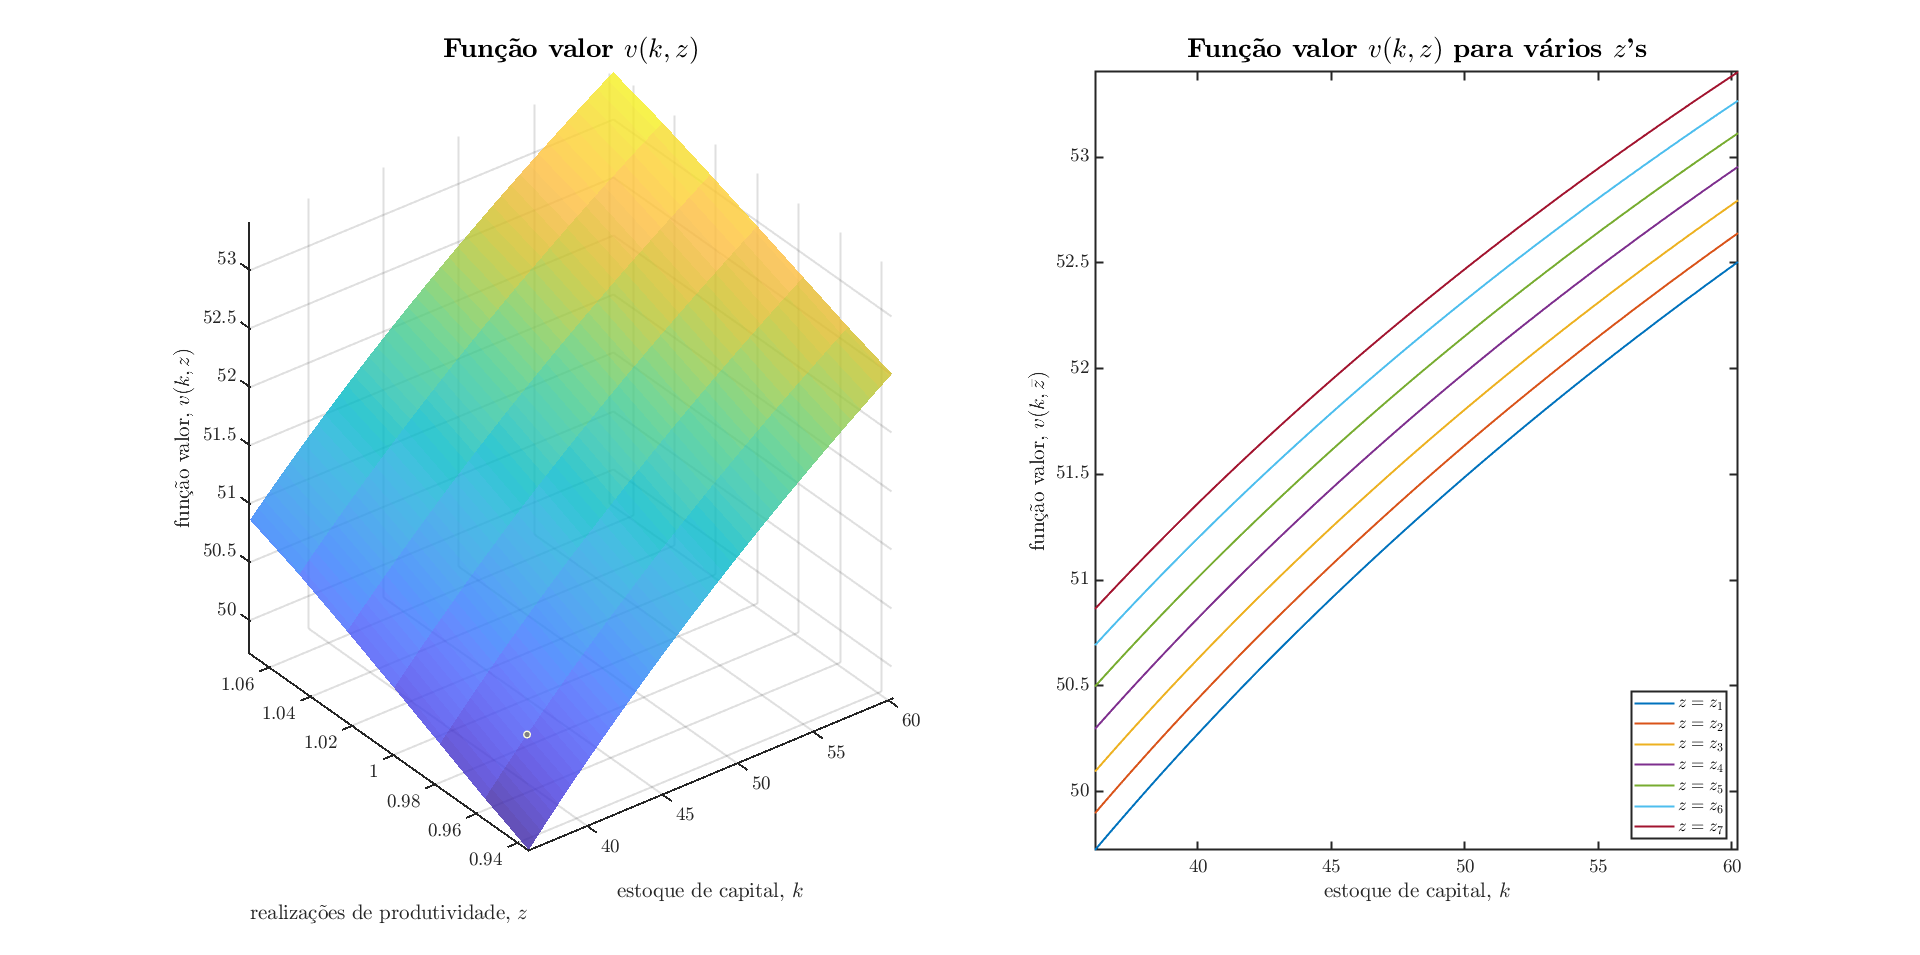
\includegraphics[scale=0.3]{value_function_brute_force_500.png}
\caption{Função Valor em 2d e 3d (500 pontos)}
\label{fig1}
\end{figure}\\
Note que a função valor obtido é de fato suave e côncava (como era de se esperar). Agora, podemos obter as funções políticas do capital e do consumo. Graficamente, temos:
\begin{figure}[htp!]
\centering
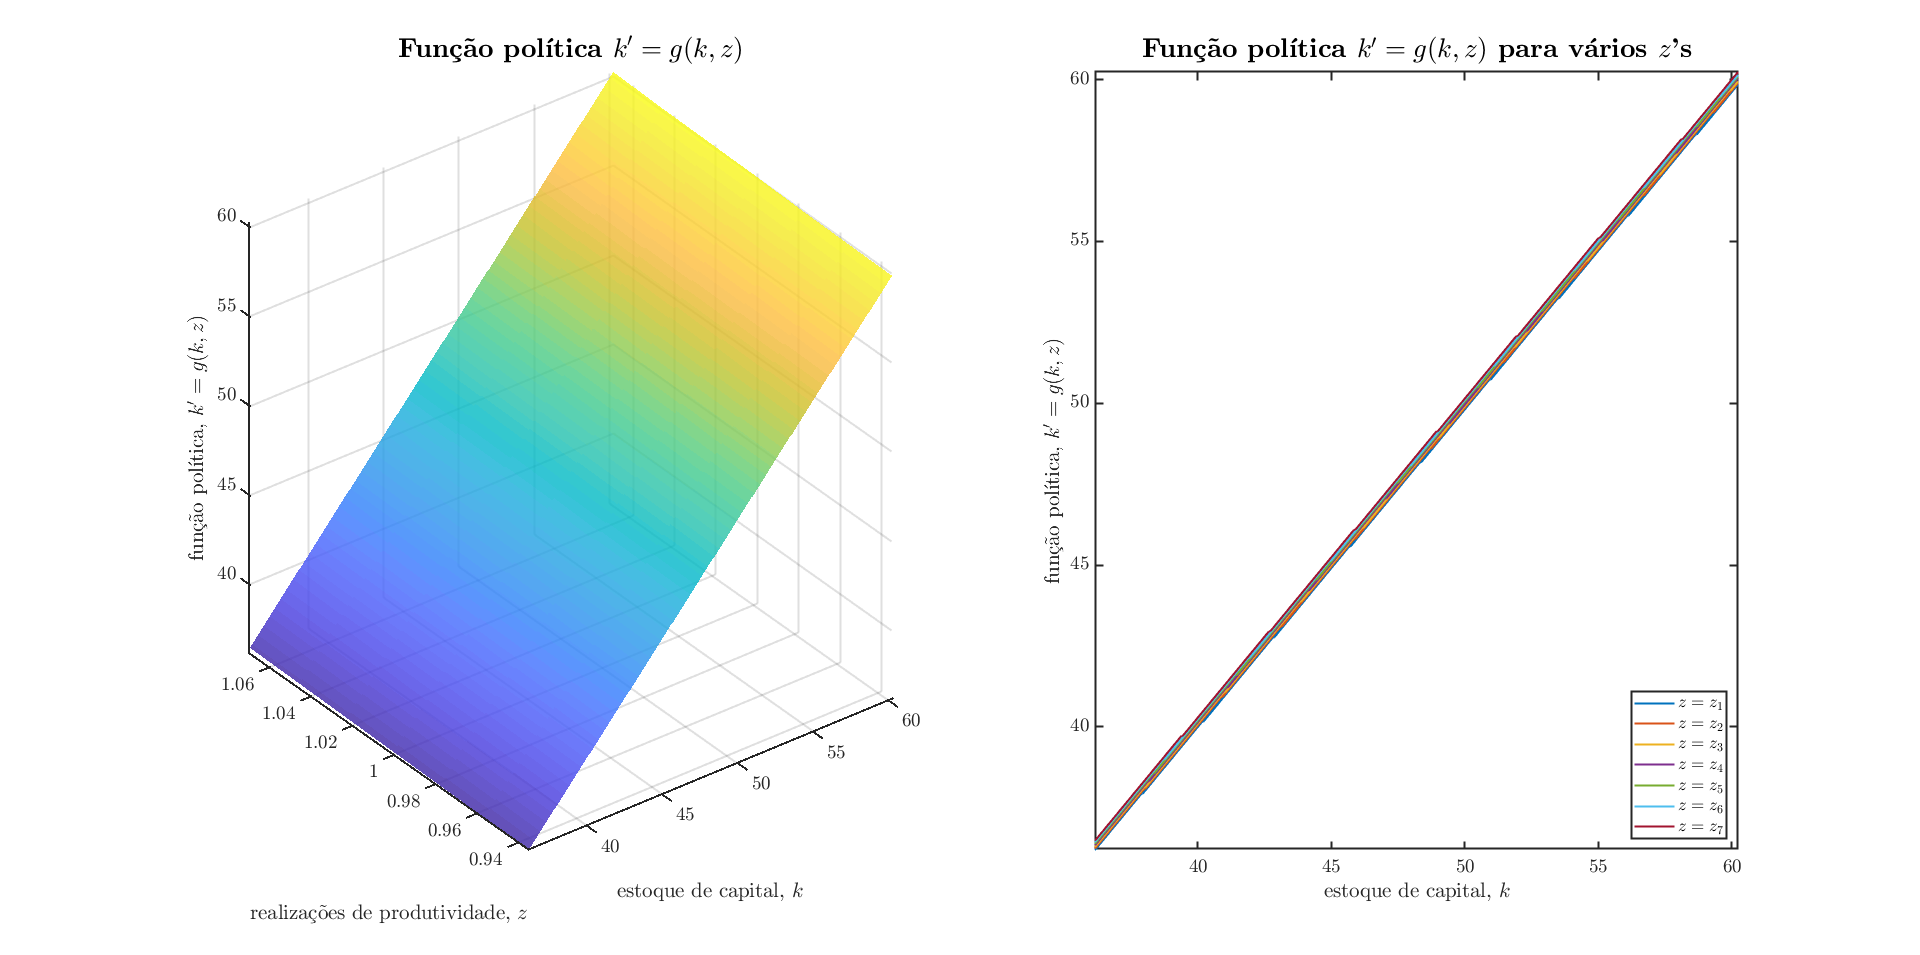
\includegraphics[scale=0.3]{capital_policy_function_brute_force_500.png}
\caption{Função política do capital em 2d e 3d (500 pontos)}
\label{fig2}
\end{figure}\\
A função política para o capital é crescente e respeita a monotonicidade. É possível ver no código o teste de monotonicidade (ifelse) que mostra que de fato os valores são maiores ou iguais que o anterior subsequente. 

\newpage

A função política para o consumo, disponível na Figura \ref{fig3}, tem um comportamento crescente (conforme esperado), apesar de apresentar kinks que não foi discutido em aula o porquê desse comportamento.

\begin{figure}[htp!]
\centering
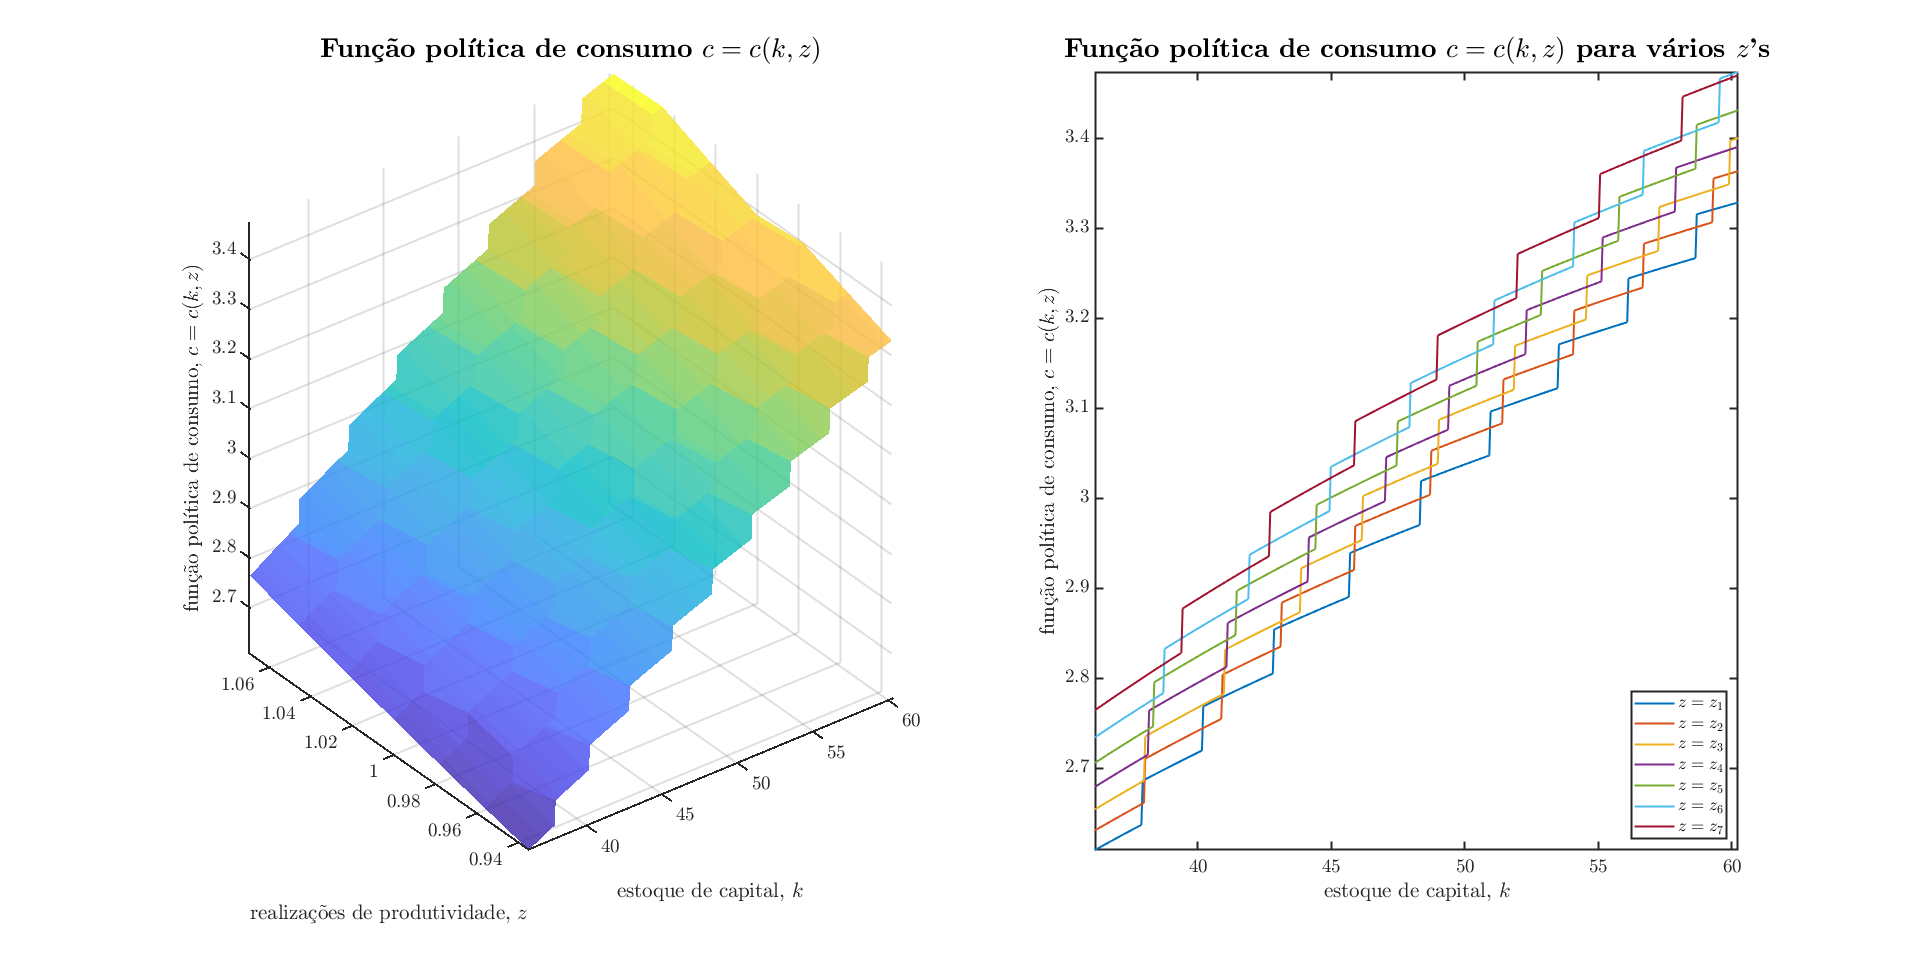
\includegraphics[scale=0.3]{consumption_policy_function_brute_force_500.png}
\caption{Função política do consumo em 2d e 3d (500 pontos)}
\label{fig3}
\end{figure}


Por fim, podemos calcular os Erros de Euler obtidos pela fórmula: 
\begin{align*}
EEE(k,z) = \log10 \left| 1 - \frac{u'^{-1}\left(\beta \E_z \left[u'(c(k'(k,z),z')) \cdot \left(1-\delta + \alpha z' k'(k,z)^{\alpha - 1}\right)\right]\right)}{c(k,z)}\right|
\end{align*}
Essa função foi implementada no arquivo \texttt{euler\_equation\_erros.m}. Graficamente, temos:
\begin{figure}[htp!]
\centering
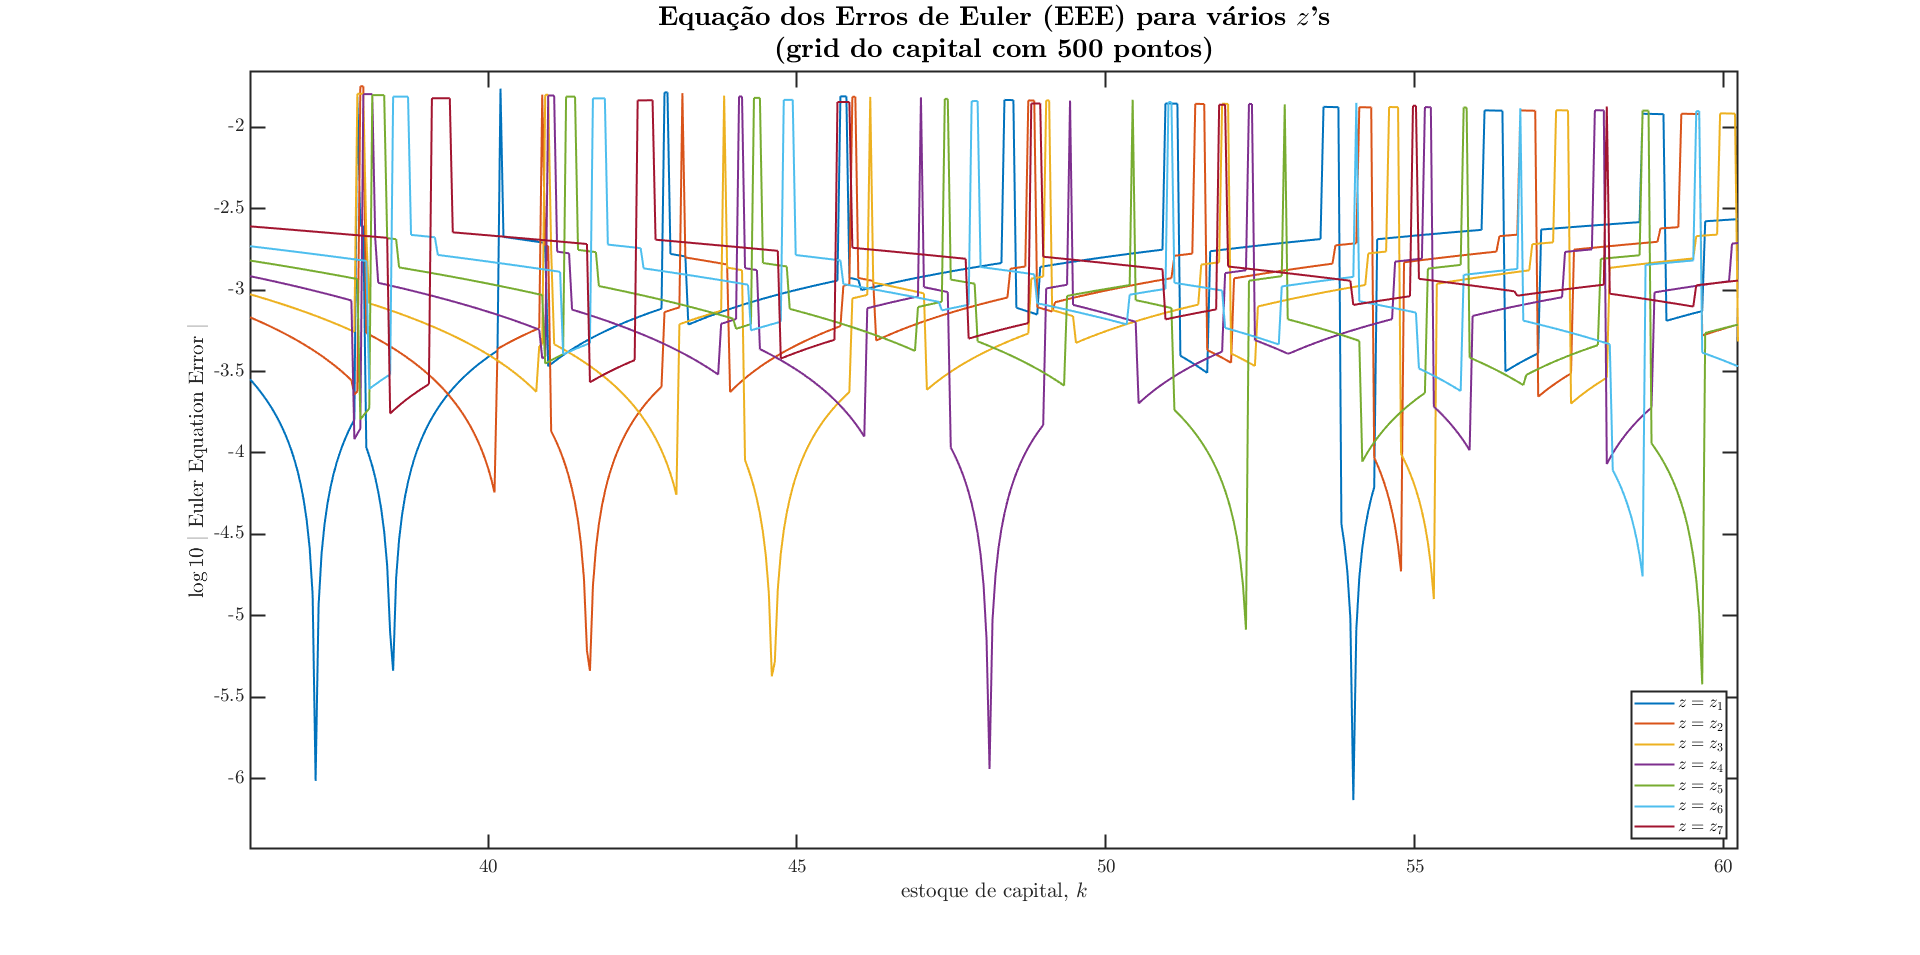
\includegraphics[scale=0.3]{eee_500.png}
\caption{Erros de Euler}
\label{fig4}
\end{figure}\\
Note que os erros de Euler variam entre $-1.7476$ e $-6.1323$. Uma interpretação interessante e de fácil compreensão equivale dizer que cometemos erros de $\$1$ a cada  $\sim \$ 55 - \$ 1,356,000$ gastos.

\newpage

Por fim, podemos mostrar que os modelos de fato geram os mesmos resultados. Eu dividi os modelos da seguinte forma: 

\begin{itemize}
\item Modelo 1: Iteração pela força bruta (\texttt{idx1});
\item Modelo 2: Iteração usando monotonicidade (\texttt{idx3}); 
\item Modelo 3: Iteração usando concavidade (\texttt{idx5}); 
\item Modelo 4: Iteração usando tanto concavidade quanto monotonicidade (\texttt{idx7}).
\end{itemize}

Para verificar se são iguais, podemos rodar o seguinte código (exemplo com o modelo de monotonicidade): \vspace{-0.5cm}
\begin{lstlisting}
% As matrizes de indices sao iguais?
igualdade = isequal(idx1,idx3);
if igualdade == 1; teste = 'iguais'; else; teste = 'diferentes'; end
fprintf('As matrizes de índices dos modelos de Brute Force e Monotonicidade são %s. \n\n', teste);
\end{lstlisting}
O output para os quatro modelos é: 
\begin{itemize}
\item As matrizes de índices dos modelos de Brute Force e Brute Force são iguais. 
\item As matrizes de índices dos modelos de Brute Force e Monotonicidade são iguais. 
\item As matrizes de índices dos modelos de Brute Force e Concavidade são iguais.
\item As matrizes de índices dos modelos de Brute Force e Concavidade com Monotonicidade são iguais.
\end{itemize}

Outra forma de comparar os modelos é computando o tempo que eles levam. A tabela abaixo fornece essa evidência (note que isso pode variar a depender do seu computador, nível de bateria, versão do matlab, etc): \vspace{-0.3cm}
\begin{lstlisting}
Method 1. Iteration of Value Function (Brute Force) 

Time (in seconds)      = 17.945 
Number of iterations   = 235 
Error                  = 0.0000099128

Method 2. Iteration of Value Function (Monotonicity) 

Time (in seconds)      = 6.658 
Number of iterations   = 235 
Error                  = 0.0000099128 

Method 3. Iteration of Value Function (Concavity) 

Time (in seconds)      = 38.965 
Number of iterations   = 235 
Error                  = 0.0000099128 

Method 4. Iteration of Value Function (Monotonicity & Concavity) 

Time (in seconds)      = 1.152 
Number of iterations   = 235 
Error                  = 0.0000099128  
\end{lstlisting}

\end{sol}


\item Para este item, refaça o item anterior usando o acelerador. Isto é, só realize a maximização em algumas iterações (10\% delas, por exemplo).
Compare os resultados com o item anterior.
\begin{sol}
No processo de iteração anterior sofre muito com o uso excessivo do operador \texttt{max} e, por isso, demanda mais tempo para processar. Howard (Howard’s Policy Iteration Algorithm) propôs um método em que você só aplica o operador em alguma iterações, isso traz eficiência para o modelo. O algoritmo seria o seguinte: 

\begin{enumerate}[wide]

\item Definimos em um ifelse as iterações que calcularemos a função valor à mão (isto é, usando o método da força bruta) e as que não utilizaremos. A sugestão do exercício é que iteremos na mão toda vez que a a variável \texttt{iter} dividida por 10 retorne resto zero, pois assim estaremos utilizando a força bruta em 10\% das vezes. No entanto, conforme comentado em sala, isso não é sempre a melhor opção. A melhor opção mesmo é você utilizar a força bruta em algumas primeiras iterações (digamos 50) e depois iteração na mão a cada 10. Esse problema foi evidenciado quando tratarmos do multigrid (lá quando utilizamos o acelerador e só iteramos em 10\%, a convergência da matriz de índices não é igual). Para resolver isso, bastar iterarmos à mão uma proporção do número de estados para o capital (escolhi 2\%, então com $\texttt{kgrid} = 500$ eu itero nas 10 primeiras a mão e com $\texttt{kgrid} = 5000$ eu itero nas 50 primeiras à mão). Logo, nesse exercício eu itero à mão as 10 primeiras vezes e depois a cada 10 itero uma. Isso é uma forma de ``policiar'' o nosso guess inicial.


\item Nas demais iterações, utilizamos o $k'$ que encontramos na última iteração obtida pela força bruta e atualizamos o Tv. Pelos slides, isso pode ser feito pois, de vez em quando, no modelo de força bruta enquanto estamos atualizando a função valor, a função política não se altera. Logo, esse procedimento pode ser feito.

\item Por fim, pararemos o loop quando batermos no número de iterações pré-definido (\texttt{max\_iter = 5000}) ou quando o \texttt{error < tol}.   

\end{enumerate} 


Agora, precisamos comparar com os resultados do item anterior. Uma forma de fazermos isso é comparar as matrizes de índices obtidas por esse método e também comparar o tempo em que eles levam para convergir. As matrizes de índices serão iguais em todos. Chamei os modelos da seguinte forma:

\begin{itemize}
\item Modelo 1.1: Iteração pela força bruta (\texttt{idx1});
\item Modelo 1.2: Iteração pela força bruta c/ Acelerador (\texttt{idx2});
\item Modelo 2.1: Iteração usando monotonicidade (\texttt{idx3}); 
\item Modelo 2.2: Iteração usando monotonicidade c/ Acelerador (\texttt{idx4}); 
\item Modelo 3.1: Iteração usando concavidade (\texttt{idx5}); 
\item Modelo 3.2: Iteração usando concavidade c/ Acelerador (\texttt{idx6}); 
\item Modelo 4.1: Iteração usando tanto concavidade quanto monotonicidade c/ Acelerador (\texttt{idx7}).
\item Modelo 4.2: Iteração usando tanto concavidade quanto monotonicidade c/ Acelerador (\texttt{idx8}).
\end{itemize}

A título de exemplo, comparo o Modelo 1.1 com o Modelo 1.2 da seguinte forma: \vspace{-0.3cm}
\begin{lstlisting}
% As matrizes de índices são iguais?
igualdade = isequal(idx1,idx2);
if igualdade == 1; teste = 'iguais'; else; teste = 'diferentes'; end
fprintf('As matrizes de índices dos modelos de Brute Force e Brute Force com Acelerador são %s. \n\n', teste);
\end{lstlisting}

\newpage

O output dos 4 modelos (comparados com o brute force original) são:
\begin{itemize}
\item As matrizes de índices dos modelos de Brute Force e Brute c/ Acelerador Force são iguais. 
\item As matrizes de índices dos modelos de Brute Force e Monotonicidade c/ Acelerador são iguais. 
\item As matrizes de índices dos modelos de Brute Force e Concavidade c/ Acelerador são iguais.
\item As matrizes de índices dos modelos de Brute Force e Concavidade com Monotonicidade c/ Acelerador são iguais.
\end{itemize}

Como resultado, todos os oito modelos geram os mesmos gráficos e resultados. A diferença se dá no tempo em que cada um leva. Note que o ganho com o acelerador é extramente expressivo quando comparado com os modelos sem acelerador.  A seguir apresento os 4 modelos com acelerador embutido:

\begin{lstlisting}
Method 1.2 Iteration of Value Function (Brute Force w/ Accelerator) 

Time (in seconds)      = 1.533 
Number of iterations   = 236 
Error                  = 0.0000098639 

Method 2.2 Iteration of Value Function (Monotonicity w/ Accelerator) 

Time (in seconds)      = 1.187 
Number of iterations   = 235 
Error                  = 0.0000099891 

Method 3.2 Iteration of Value Function (Concavity with Accelerator) 

Time (in seconds)      = 5.295 
Number of iterations   = 235 
Error                  = 0.0000099890 

Method 4.2 Iteration of Value Function (Monotonicity & Concavity with Accelerator) 

Time (in seconds)      = 0.826 
Number of iterations   = 235 
Error                  = 0.0000099129
\end{lstlisting}




A tabela a seguir resume o resultado dos 8 modelos especificados:
\begin{table}[htp!]
\caption{Tabela de tempos (em segundos)}

\centering
\begin{tabular}{>{\raggedright\arraybackslash}p{7cm}>{\centering\arraybackslash}p{3cm}>{\centering\arraybackslash}p{3cm}>{\centering\arraybackslash}p{3cm}}
                                                          & Sem Acelerador         & Com Acelerador         & Ganho                  \\
Modelo 1. Brute Force                                     & 17.945                 & 1.533                  & 91\%                  \\
Modelo 2. Monotonicidade                                  & 6.658                  & 1.187                  & 82\%                  \\
Modelo 3. Concavidade                                     & 38.965                 & 5.295                  & 86\%                  \\
{Modelo 4. Monotonicidade   e Concavidade} & {1.152} & {0.086} & {93\%} \\
                                                          &                        &                        &                       
\end{tabular}
\end{table}
Por fim, os erros de euler também serão iguais ao item anterior, uma vez que para seu cálculo utilizamos apenas o consumo e capital que, como são os mesmos, gerarão resultados idênticos.
\end{sol}

\newpage

\item Para este item, refaça o problema usando múltiplos grids (\textit{multigrid}). Primeiro, resolva o problema usando um grid de 100 pontos, depois 500 e, finalmente, 5000. Para cada grid posterior, utilize a solução anterior como chute inicial (você precisará interpolar). Compare com os itens anteriores.
\begin{sol}
A ideia desse método é resolver o problema num grid mais ``grosso'' e usa esse resultado como guess inicial a partir de um grid mais ``fino'' obtido por meio de interpolação da função valor obtida no problema com grid mais ``grosso''. 

O algoritmo para o caso específico do exercício pode ser resumido da seguinte forma:

\begin{enumerate}[wide]

\item Primeiro, definimos um multigrid conforme enunciado e montamos um loop pequeno que percorre os três grids. 

\item Agora, resolvemos o problema para cada um desses grids, sendo que começamos com o mais grosso e interpolando a função valor para obter como guess inicial para os grids mais finos. 
Note que para o grid mais grosso de todos também utilizamos o guess inicial do Benjamin Moll (não ajuda muito porque é um grid de 100 pontos, mas se fosse com mais pontos, esse guess inicial pode ajudar a iterar mais rápido no primeiro grid).

\item Esse chute inicial que vai mudando ajuda o código a convergir mais rápido. Sendo assim, fazemos até o terceiro grid com 5000 elementos.

\end{enumerate} 

A função \texttt{iteration\_multigrid.m}, disponível no código anexo, aplica esse problema. Agora plotamos os gráficos obtidos desse problema. Na Figura \ref{fig5} temos o gráfico da função valor obtida pelo método da força bruta com uso do multigrid. 

\begin{figure}[htp!]
\centering
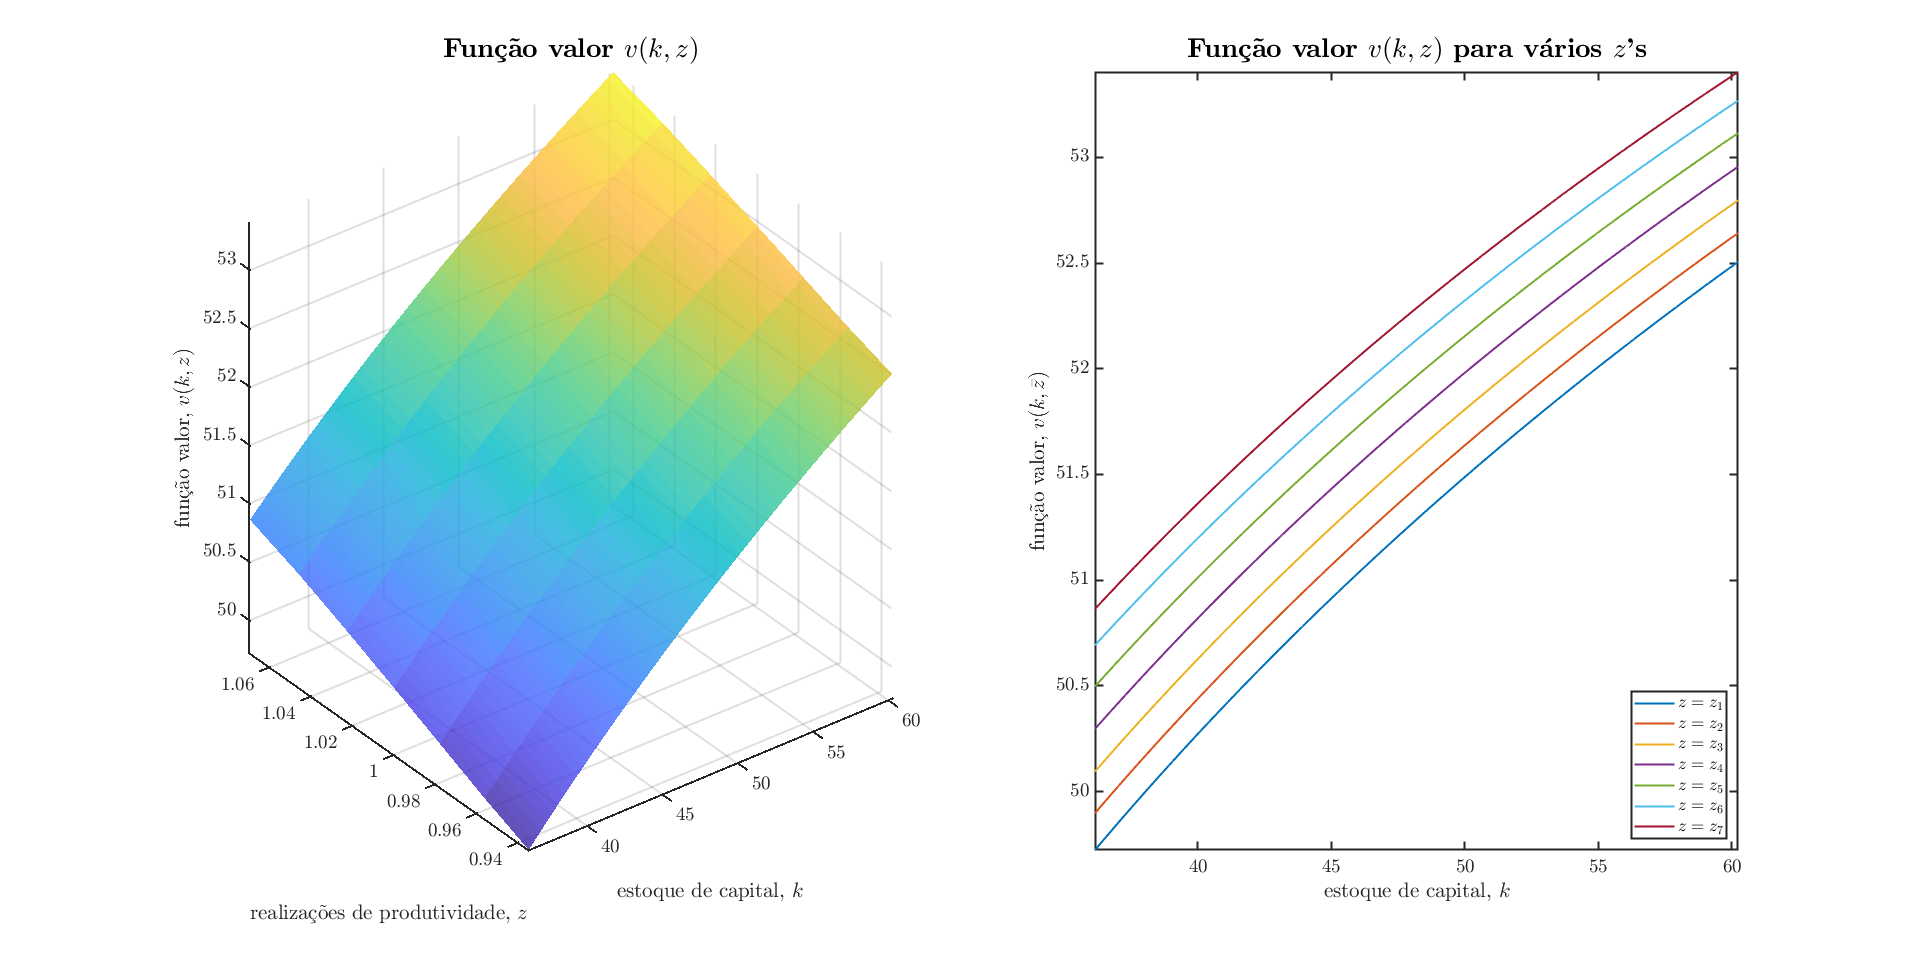
\includegraphics[scale=0.3]{value_function_brute_force_5000.png}
\caption{Função Valor em 2d e 3d (5000 pontos)}
\label{fig5}
\end{figure}



Muito próxima ao obtido com o grid de 500 pontos. Não há diferença a olho nu. Concavidade e suavidade preservadas. 

\newpage

Agora, plotamos a função política do capital obtida nesse grid mais fino. A Figura \ref{fig6} mostra o comportamento.

\begin{figure}[htp!]
\centering
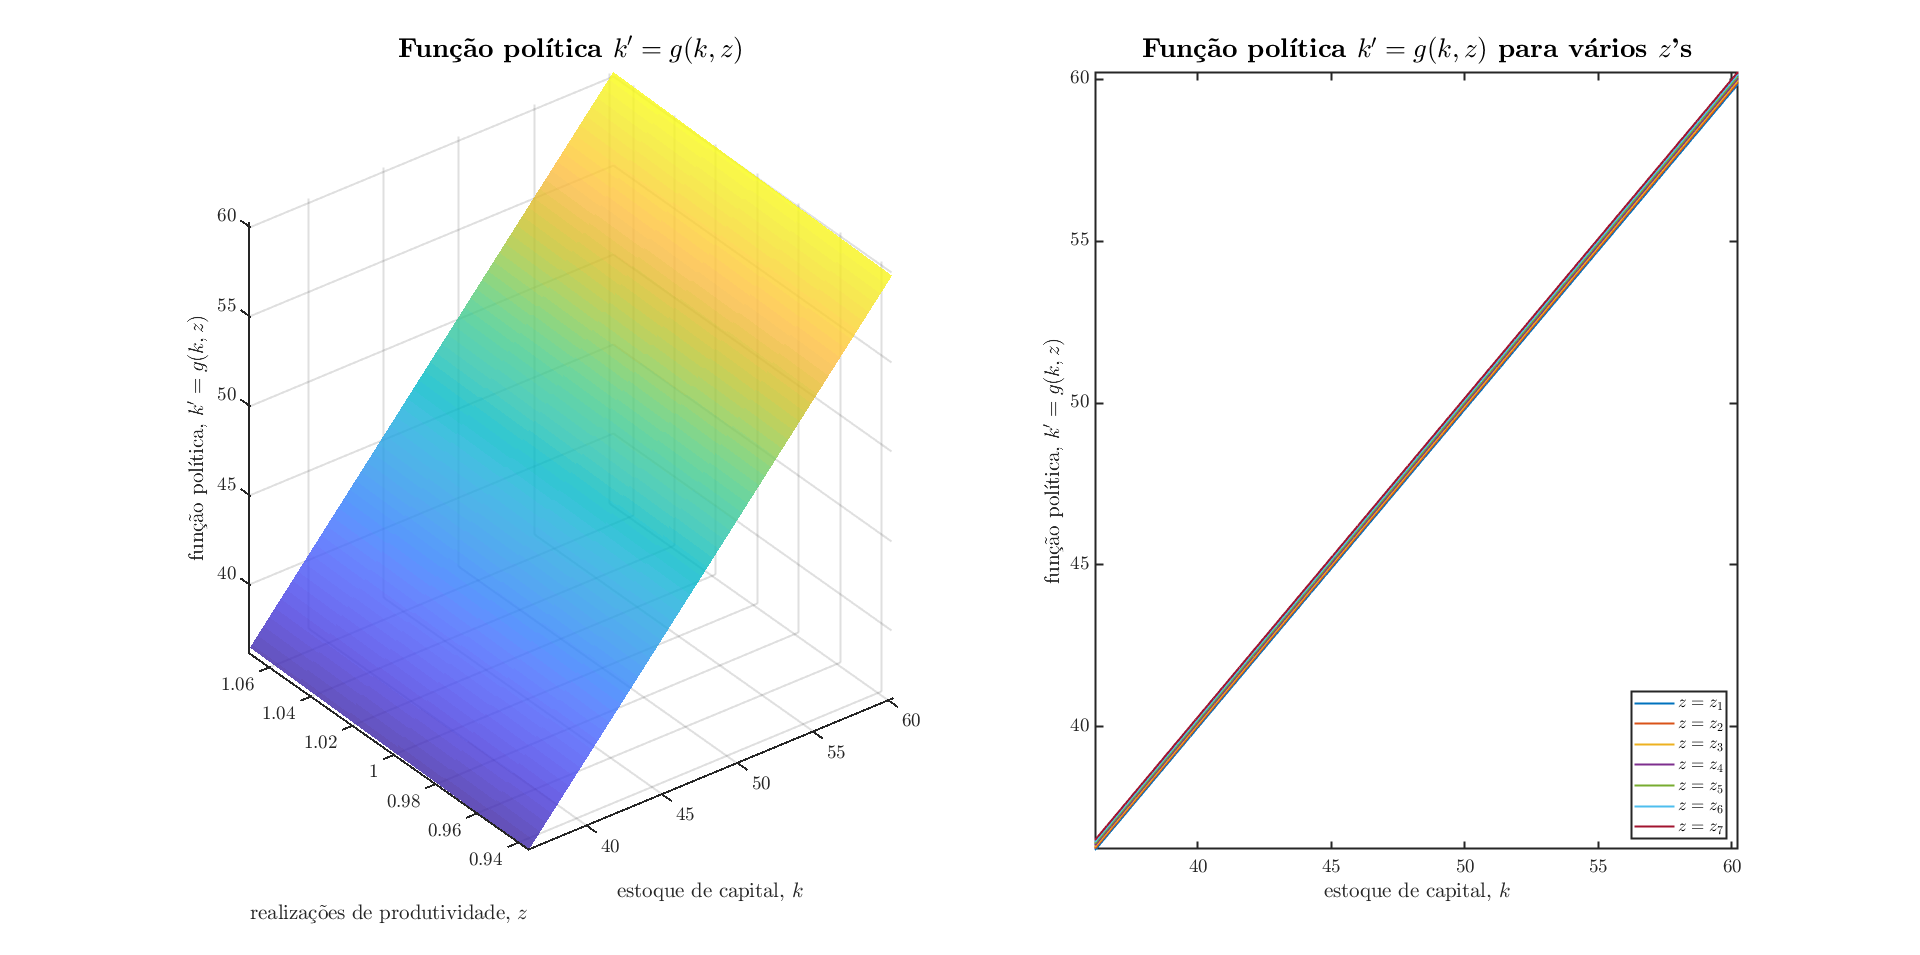
\includegraphics[scale=0.3]{capital_policy_function_brute_force_5000.png}
\caption{Função política do capital em 2d e 3d (5000 pontos)}
\label{fig6}
\end{figure}

Note que é muito parecida com aquela obtida para o grid com 500 pontos. No entanto, se dermos zoom em ambas, conseguimos verificar a diferença. A Figura \ref{fig7} apresenta esse resultado. É possível ver que com o grid mais grosso os kinks são mais frequentes.

\begin{figure}[htp!]
\centering
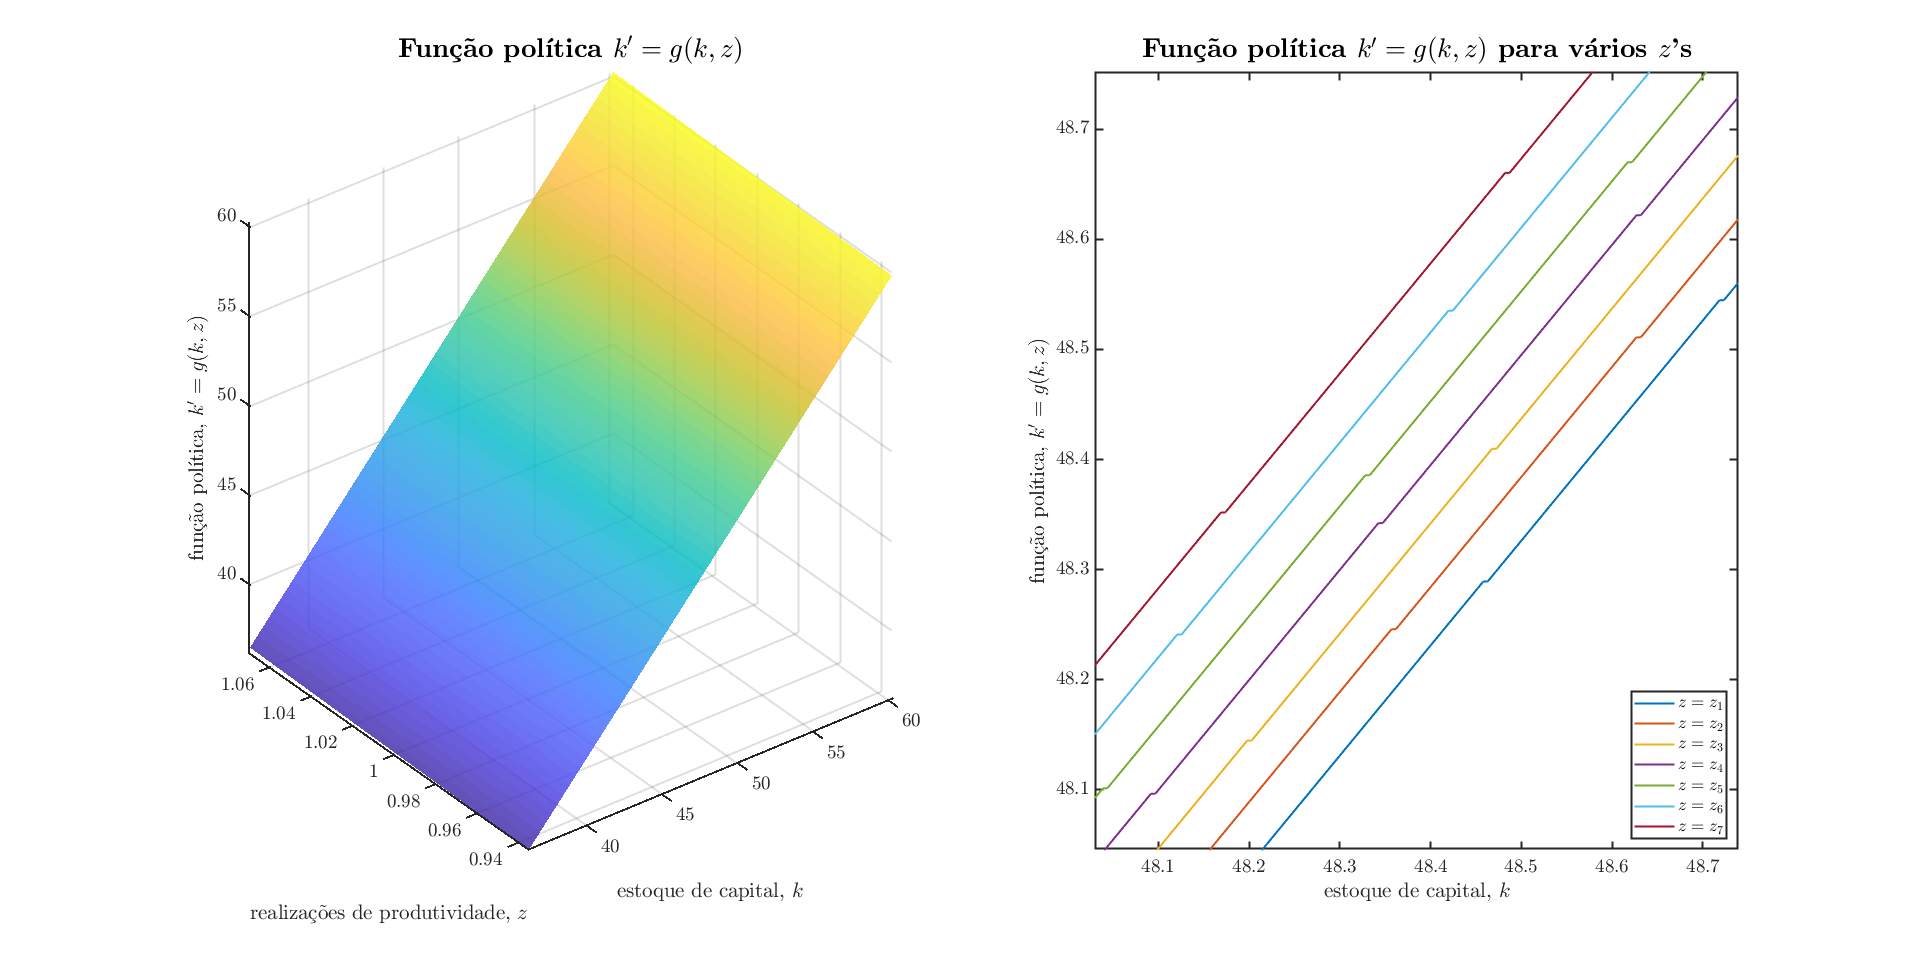
\includegraphics[scale=0.22]{capital_policy_function_brute_force_5000_zoom.png}
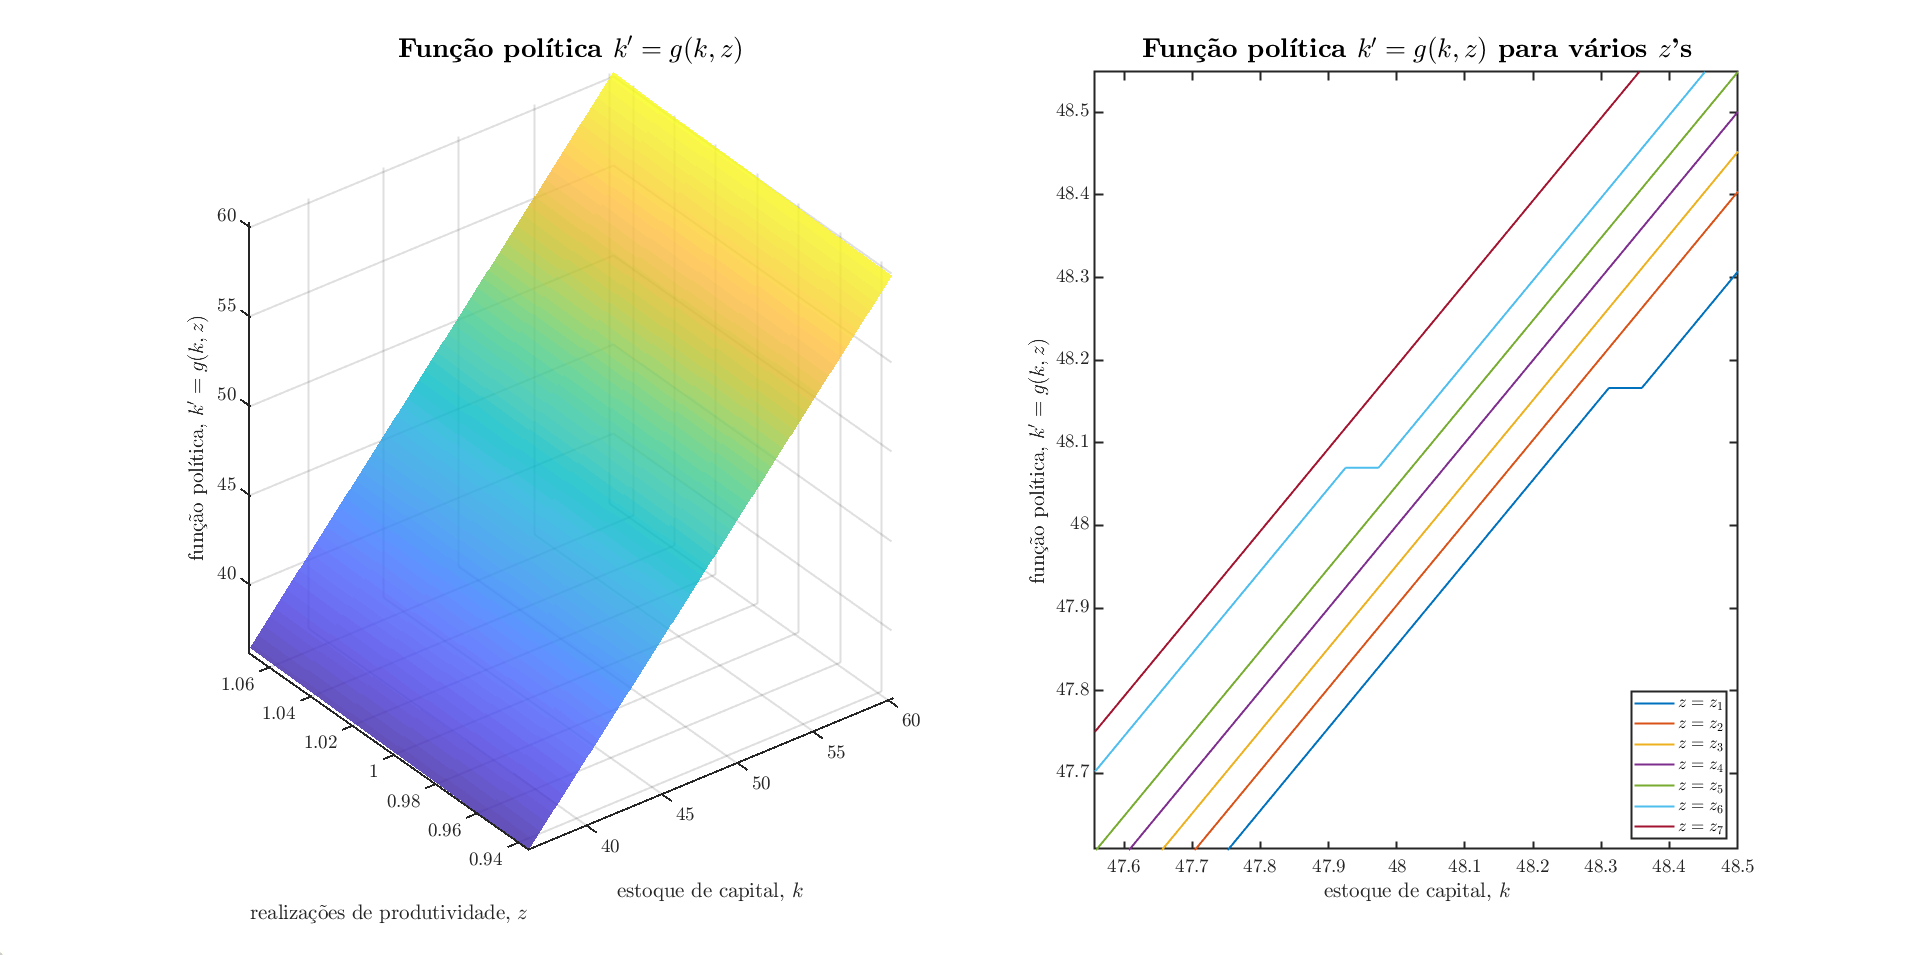
\includegraphics[scale=0.22]{capital_policy_function_brute_force_500_zoom.png}
\caption{Função política do capital em 2d e 3d (5000 pontos)}
\label{fig7}
\end{figure}

\newpage

A Figura \ref{fig8}, por sua vez, mostra a função política do consumo. Note que o consumo é muito mais suave no grid mais fino (com 5000 pontos) do que no grid mais grosso (com 500 pontos). Isso faz sentido, uma vez que estamos considerando muito mais opções de capital no grid (isso exige mais custo computacional que pode ser ``driblado'' com o suo apropriado dos outros métodos).

\begin{figure}[htp!]
\centering
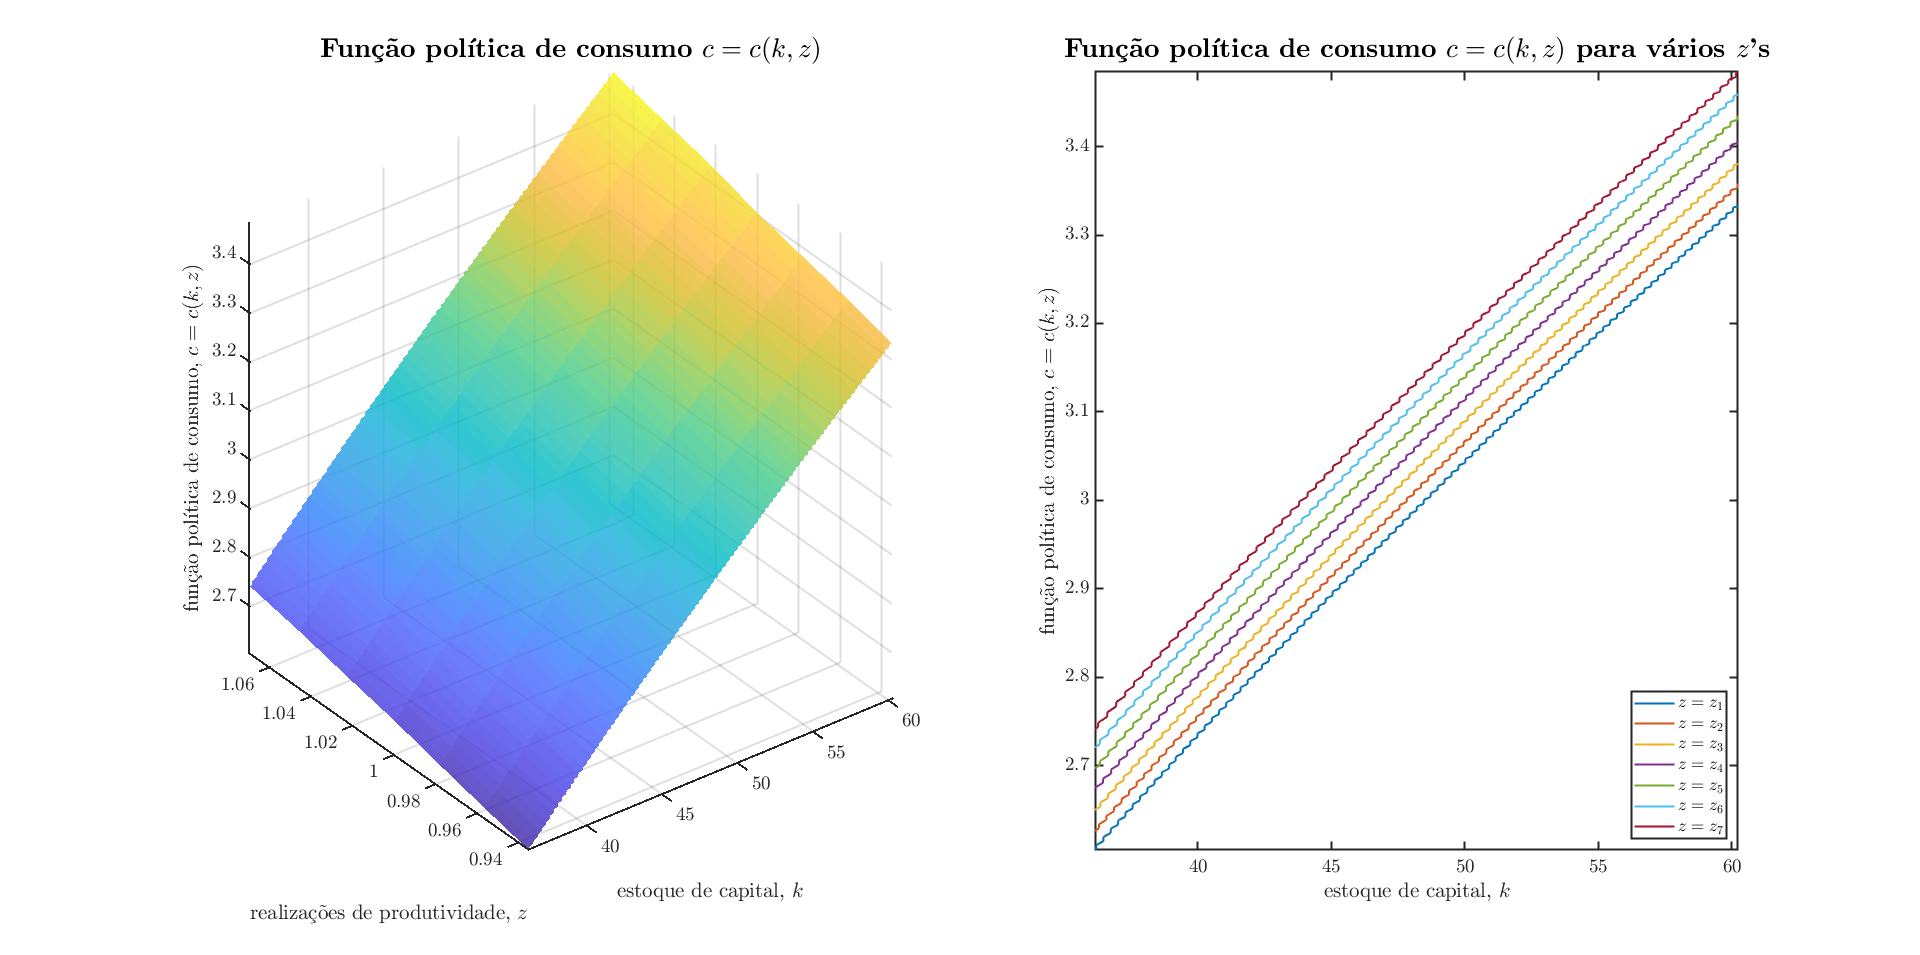
\includegraphics[scale=0.3]{consumption_policy_function_brute_force_5000.png}
\caption{Função política do consumo em 2d e 3d (5000 pontos)}
\label{fig8}
\end{figure}


Note que o mais interessante desse modelo com mais pontos são os erros de Euler que são obtidos. A diferença entre os dois é bastante perceptível e a amplitude dos valores também é maior. Nesse caso, os erros variam de $-2.7646$ a $-7.9763$ (lembre-se que no força bruta tínhamos $-1.7476$ e $-6.1323$). Note que isso evidencia um ganho de precisão muito maior do que aqueles obtidos com o grid menor (500 pontos) nos itens anteriores pois, na nossa interpretação, equivale dizer que cometemos um erro de $\$1$ a cada $~\$581.00 - \$94,689,102.46$ gastos (podemos gastar muito mais). A Figura \ref{fig9} apresenta seu comportamento.

\begin{figure}[htp!]
\centering
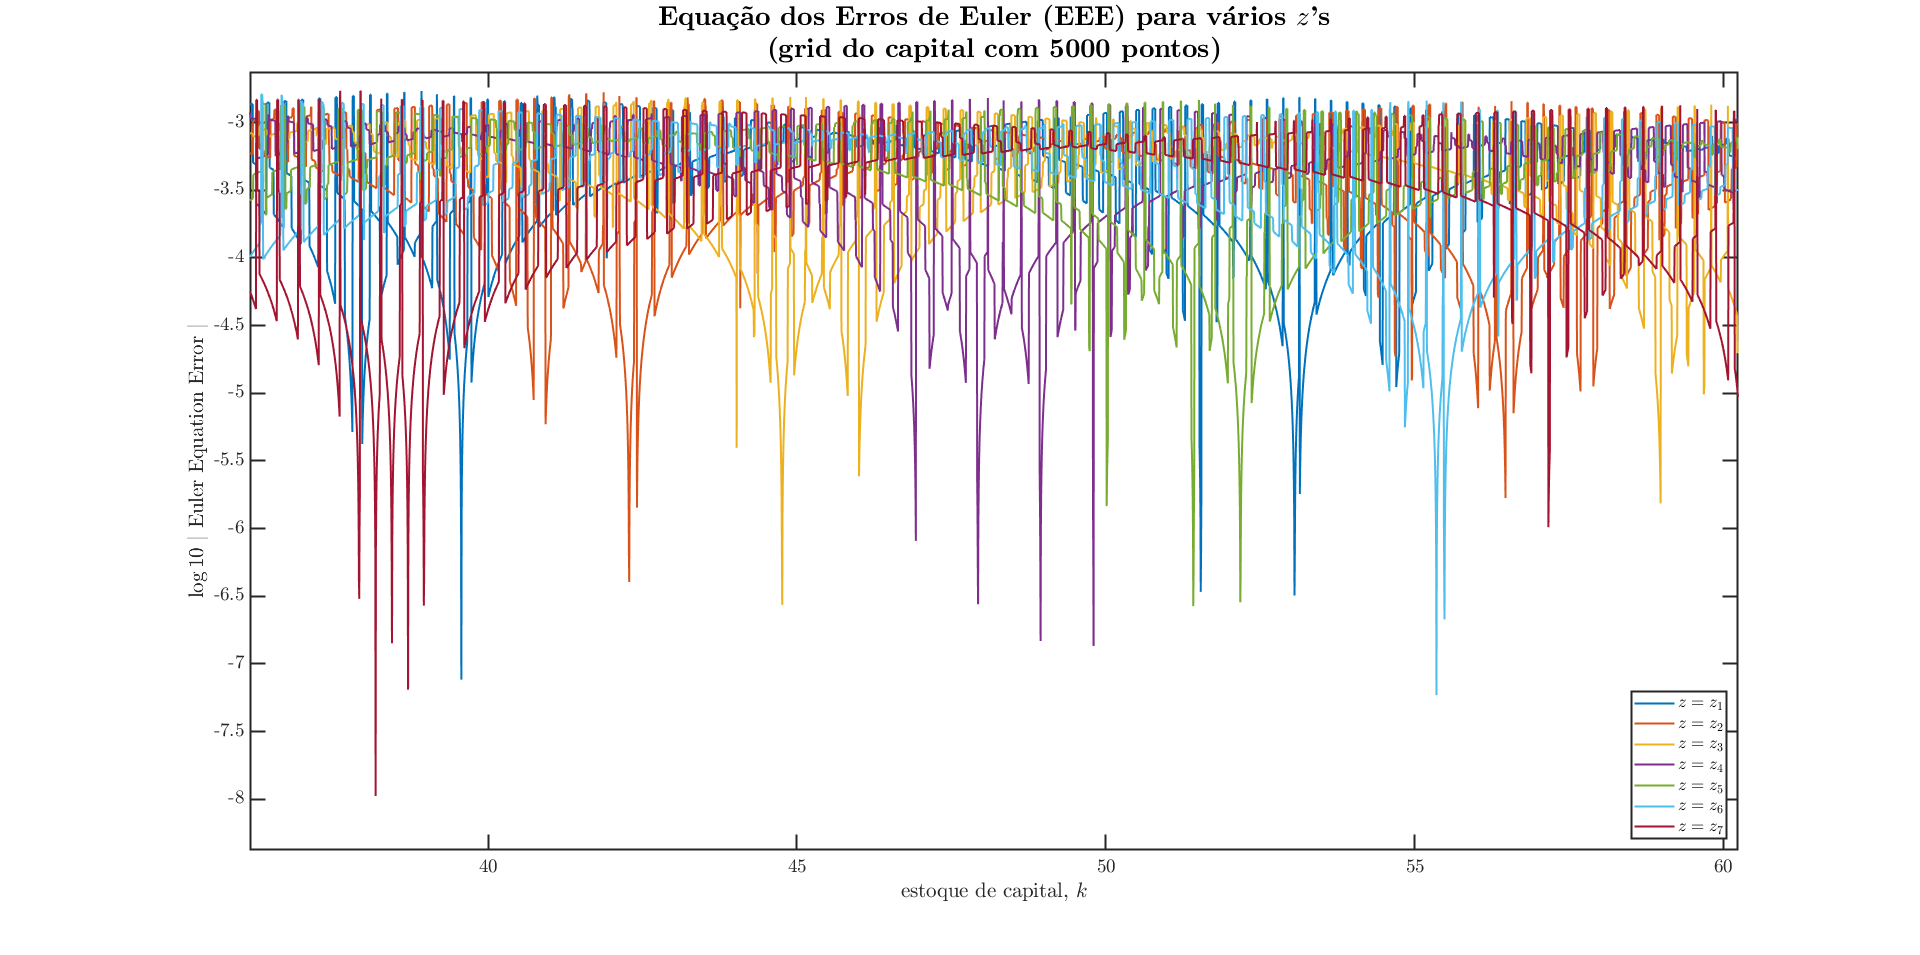
\includegraphics[scale=0.3]{eee_5000.png}
\caption{Erros de Euler (5000 pontos no grid de capital)}
\label{fig9}
\end{figure}


\newpage

Agora, verificamos o desempenho do multigrid com o uso dos diversos métodos que foram listados anteriormente. Um ponto a salientar sobre o multigrid é o uso do acelerador, quando usamos o acelerador, precisamos iterar mais vezes no ínicio, isto é, não é adequado iterar só em 10\% das vezes, pois caso façamos isso, os valores serão diferentes. Essa diferença é muito pequena, mas altera os índices na matriz de índices. Sendo assim, optei por aumentar o número de iterações no início! Mas existe um trade-off pois como estamos trabalhando com o objetivo de obter as funções num grid bem maior e o número de iterações necessárias para os grids mais finos vai caindo a medida que novos guesses são incorporados, isso deixa o acelerador mais lento. Por exemplo, no multigrid do exercício proposto, o último grid de 5000 pontos converge com apenas 50 iterações, no entanto, o acelerador percorre as 100 primeiras aplicando o máximo, logo, no último grid não há ganho em usar o acelerador ou não, mas temos ganho (ou não) para os grids mais grossos que convergem com um número maior de iterações, vai depender do número de iterações necessárias para convergir, se for menor que 100 então não há ganho, se for maior, há ganho. A seguir temos os tempos obtidos para cada método (lembre-se: existe um trade-off entre número de iterações no início com acelerador e precisão da matriz de índices).

\begin{lstlisting}
Method 1.1 Iteration of Value Function (Brute Force) - Multigrid

Time (in seconds)      = 209.1778 
Number of iterations   =  50 
Error                  = 0.0000099546 


Method 1.2 Iteration of Value Function (Brute Force w/ Accelerator) - Multigrid

Time (in seconds)      = 212.3767 
Number of iterations   =  50 
Error                  = 0.0000099546 


Method 2.1 Iteration of Value Function (Monotonicity) - Multigrid

Time (in seconds)      = 104.0027 
Number of iterations   =  50 
Error                  = 0.0000099546 


Method 2.2 Iteration of Value Function (Monotonicity w/ Accelerator) - Multigrid

Time (in seconds)      = 92.1083 
Number of iterations   =  50 
Error                  = 0.0000099546 


Method 3.1 Iteration of Value Function (Concavity) - Multigrid

Time (in seconds)      = 578.5688 
Number of iterations   =  50 
Error                  = 0.0000099546 


Method 3.2 Iteration of Value Function (Concavity with Accelerator) - Multigrid

Time (in seconds)      = 580.1528 
Number of iterations   =  50 
Error                  = 0.0000099546 

Method 4.1 Iteration of Value Function (Monotonicity & Concavity) - Multigrid

Time (in seconds)      = 10.5017 
Number of iterations   =  50 
Error                  = 0.0000099546 


Method 4.2 Iteration of Value Function (Monotonicity & Concavity with Accelerator) 

Time (in seconds)      = 10.5574 
Number of iterations   =  50 
Error                  = 0.0000099546
\end{lstlisting}

Como dito, note que nesse caso, os modelos com acelerador são (em sua maioria) mais lentos do que os modelos sem acelerador. Isso se dá por conta da escolha de iterações com o máximo. Note que o número de iterações máximo do grid mais fino são 50, no entanto, meu acelerador está configurado para acelerar só a partir de 100 iterações. Logo, não faz muita diferença entre os métodos. Uma forma de resolver isso seria mudar na função com acelerador o número de iterações iniciais, no entanto, como já mencionado, isso muda a matriz de índices. Apesar da função valor, consumo e capital não sofrer alteração visual considerável, visto que são muito valores no grid e eles são muito próximos um do outro.


\end{sol}

\item Para este item, resolva o problema usando o método do grid endógeno
(\textit{endogenous grid method}). Compare com os itens anteriores.
\begin{sol}
O algoritmo do multigrid está descrito nos slides do professor. Ele envolve o uso de diversas interpolações distintas. Basicamente, o método passa por encontrar o zero da CPO dado um certo chute para o consumo. Para isso, utilizei o método da bisecção (\texttt{bisection\_method.m}) disponível na internet no site MathWorks. O chute inicial para o consumo foi (chute natural): 
\begin{align*}
c(k,z) = zk^\alpha + (1-\delta)k - k
\end{align*}

O método foi implementado na função \texttt{iteration\_egm.m}. Ele tem como output o consumo obtido pelo método endógeno e a partir daí podemos calcular a função política do capital e a função valor. O tempo decorrido foi: 

\begin{lstlisting}
Method 5. Iteration of Value Function (Endogenous Grid) 

Time (in seconds)      = 7.426 
Number of iterations   = 175 
Error                  = 0.0000099762 
\end{lstlisting}

\newpage

Agora, plotamos os principais resultados. Primeiramente, plotamos a função valor obtida (ordem inversa só para manter raciocínio). A Figura \ref{fig10} apresenta seu comportamento. 

\begin{figure}[htp!]
\centering
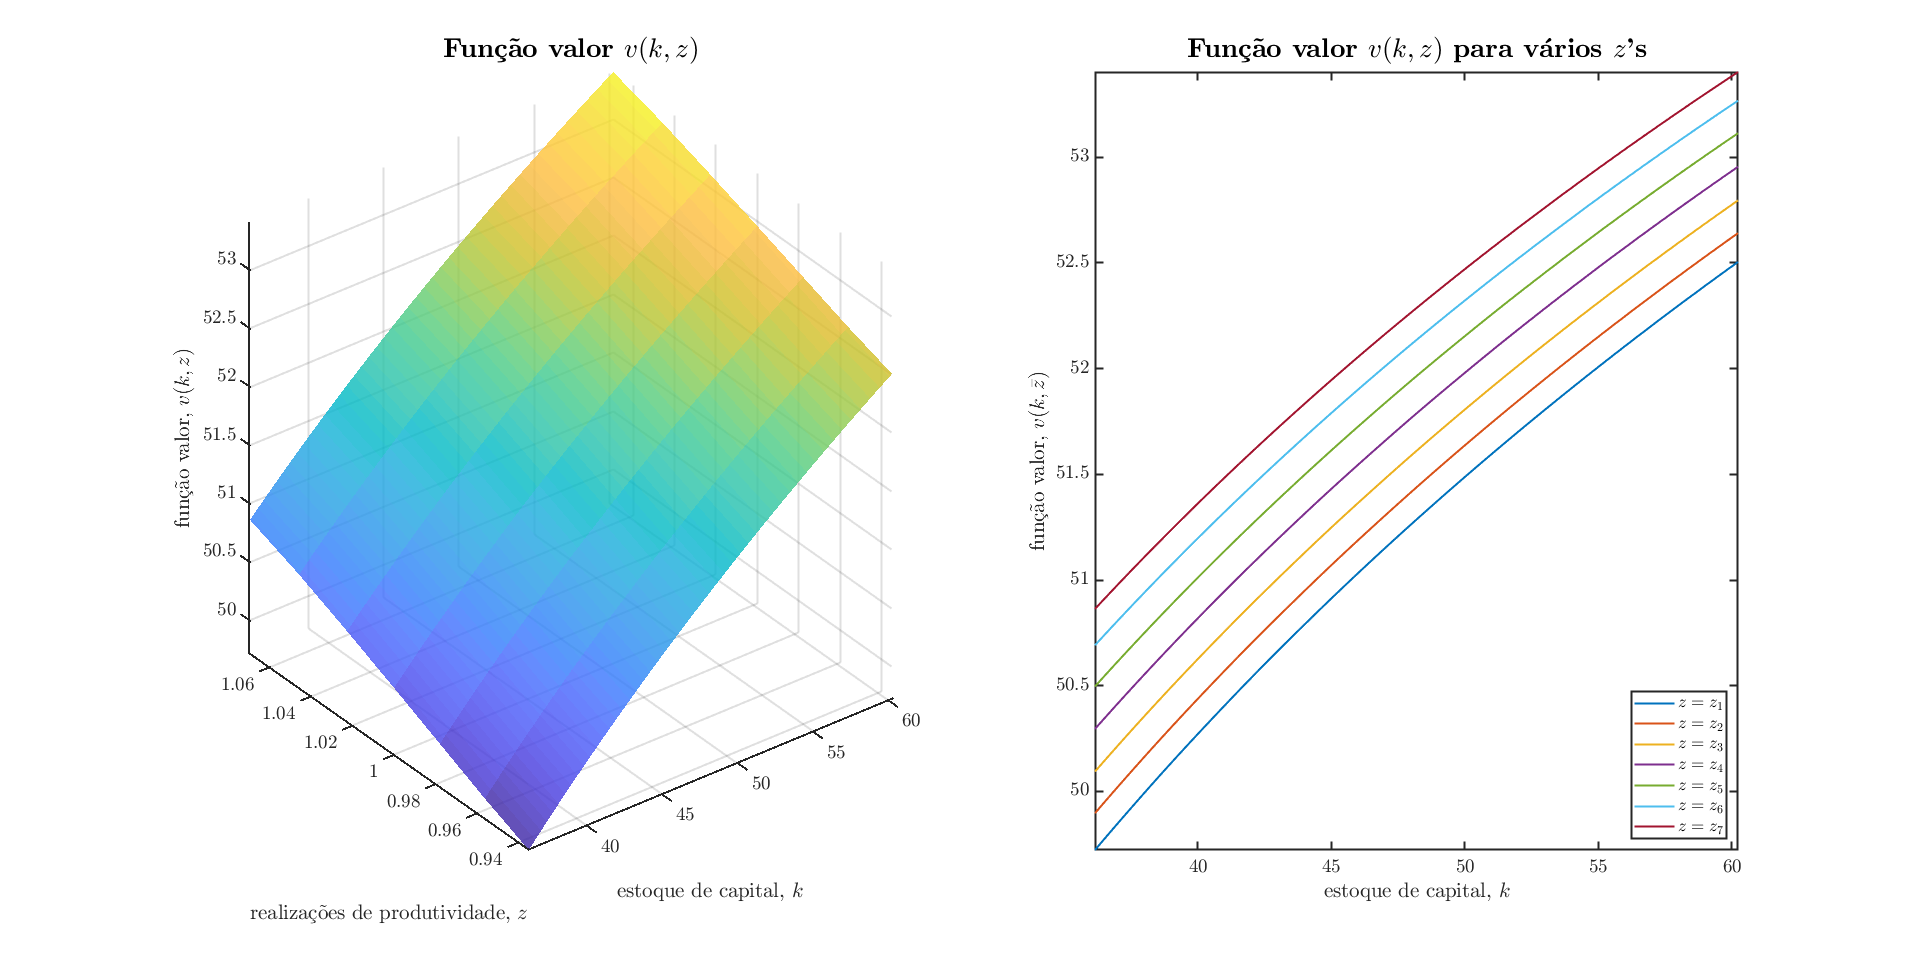
\includegraphics[scale=0.28]{value_function_egm.png}
\caption{Função valor obtida pelo método do grid endógeno}
\label{fig10}
\end{figure}
Note que apresenta um comportamento extremamente parecido com a obtido pelos métodos anteriores. A diferença é mais nas proeminente nas funções políticas como pode ser visto nas Figuras \ref{fig11} e \ref{fig12} que representam as funções políticas para o capital e consumo, respectivamente.

\begin{figure}[htp!]
\centering
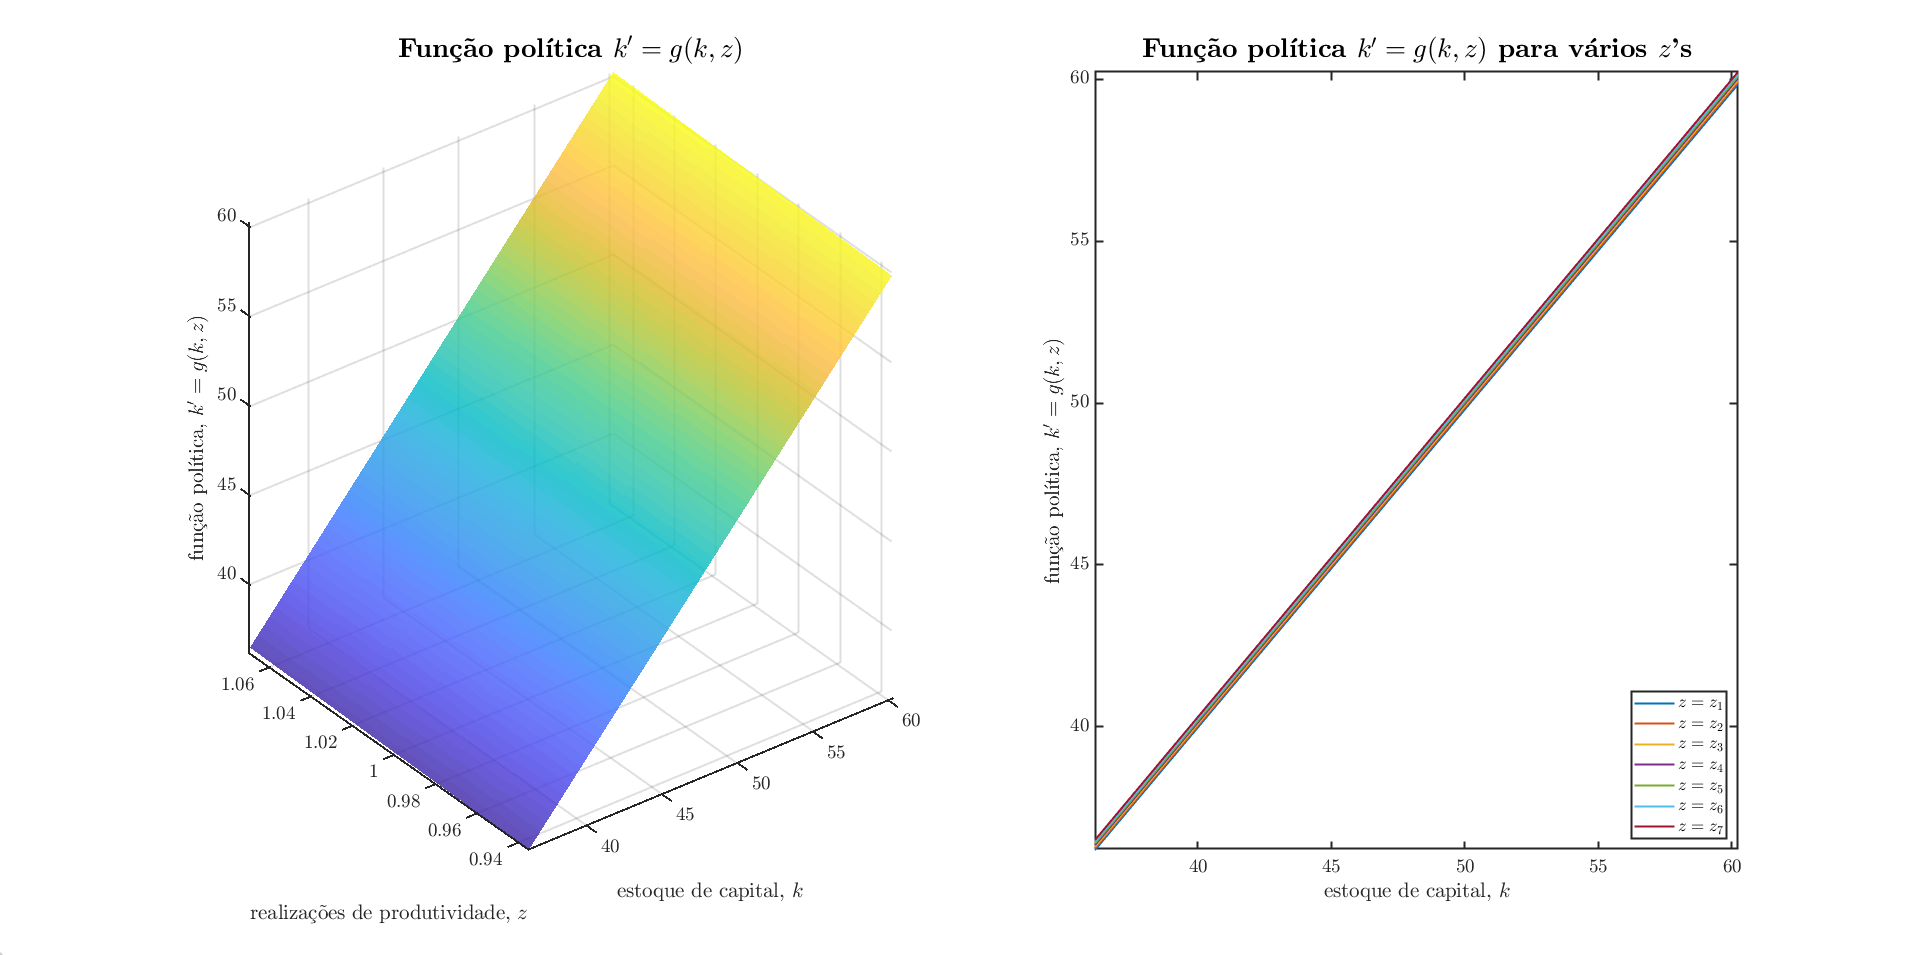
\includegraphics[scale=0.22]{capital_policy_function_egm.png}
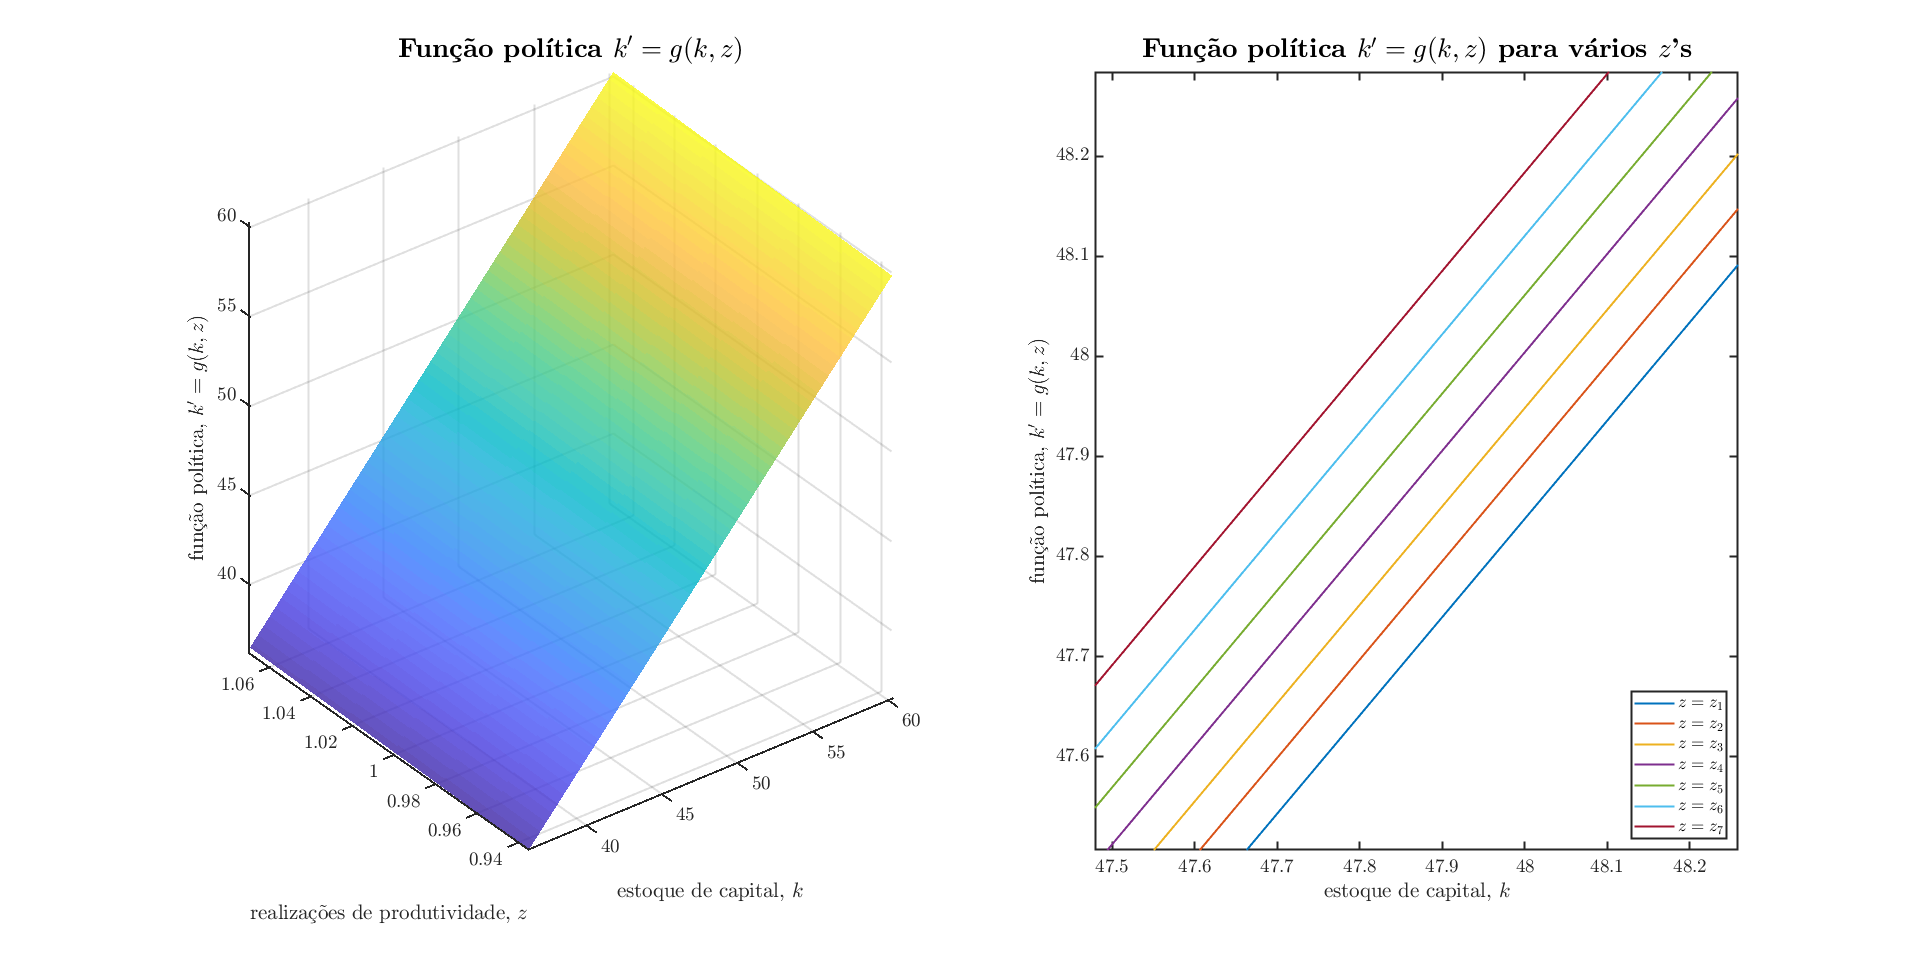
\includegraphics[scale=0.22]{capital_policy_function_egm_zoom.png}
\caption{Função política do capital obtida pelo método do grid endógeno}
\label{fig11}
\end{figure}

Note que apesar de parecidas quando não temos zoom, a função política do capital ao colocarmos zoom, passa a ser totalmente linear e sem kinks (muito mais bonita). Para o consumo, temos:

\begin{figure}[htp!]
\centering
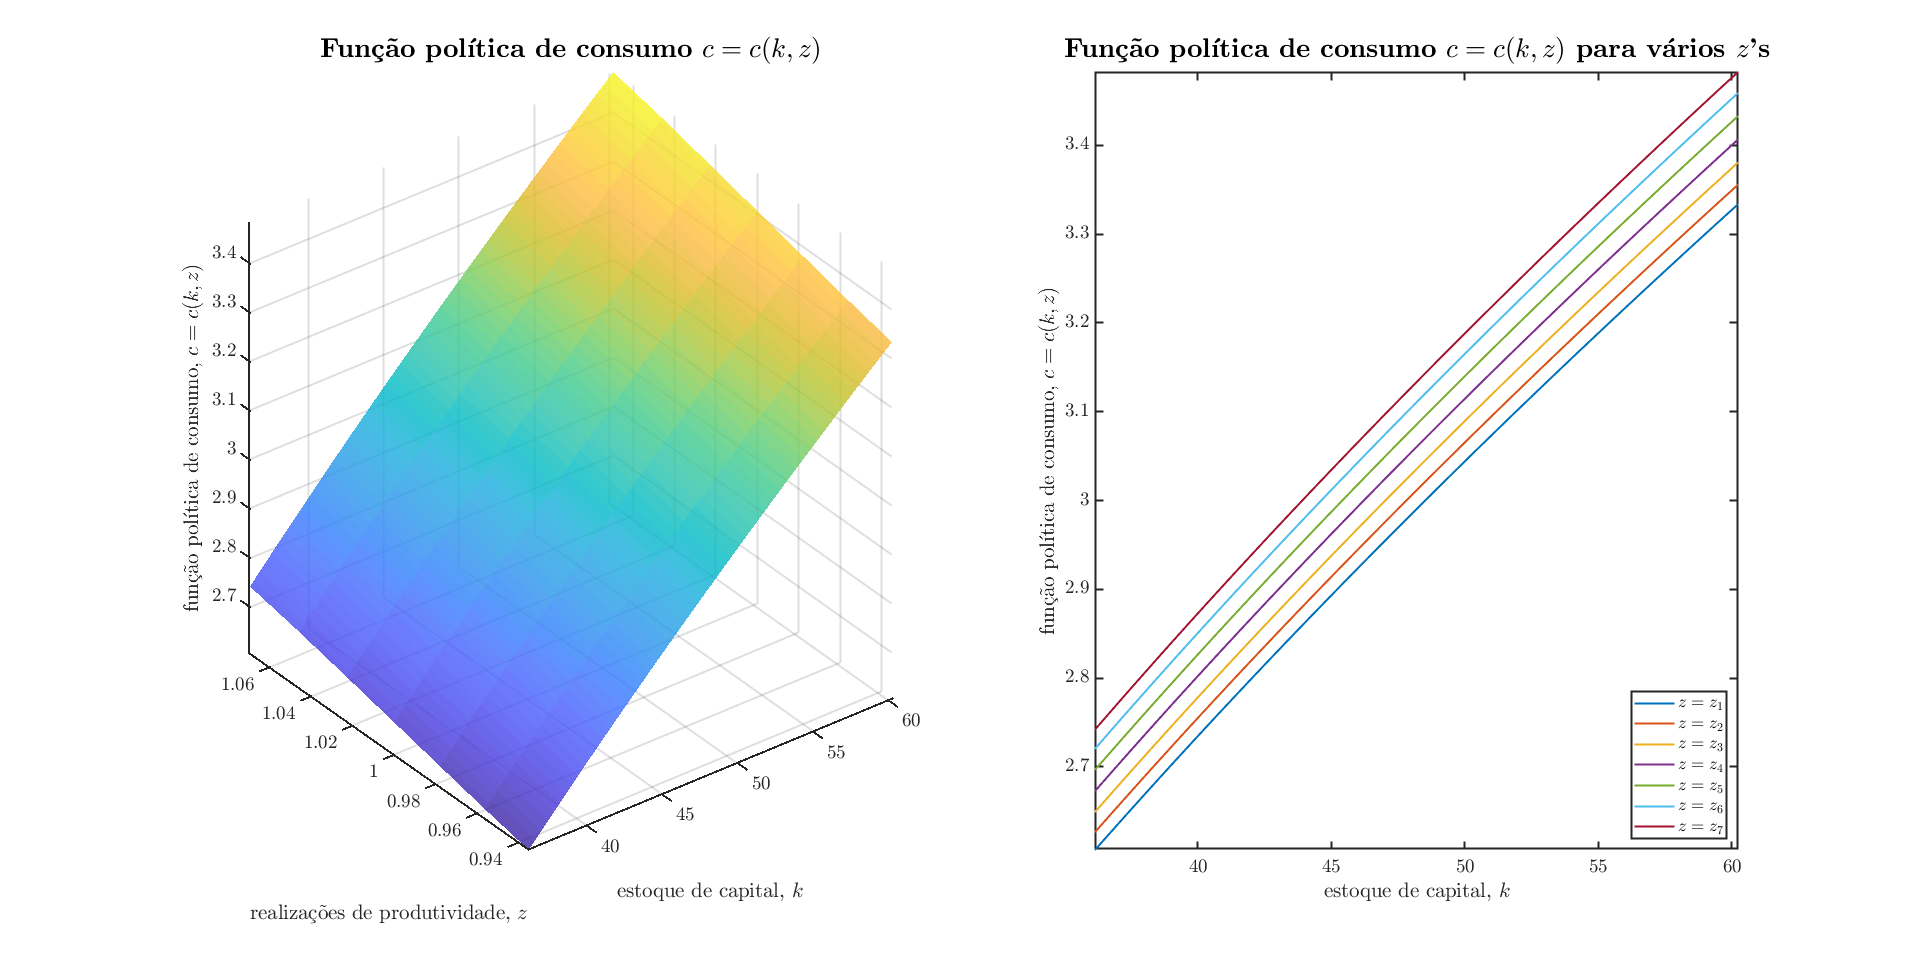
\includegraphics[scale=0.30]{consumption_policy_function_egm.png}
\caption{Função política do consumo obtida pelo método do grid endógeno}
\label{fig12}
\end{figure}
Note que a função apresenta o comportamento esperado de ser crescente e agora bastante suave, sem kinks (mesmo com zoom). Por fim, temos os erros de Euler desse modelo, implementado pela função \texttt{euler\_equation\_erros\_egm.m}. A Figura \ref{fig13} mostra seu comportamento.
\begin{figure}[htp!]
\centering
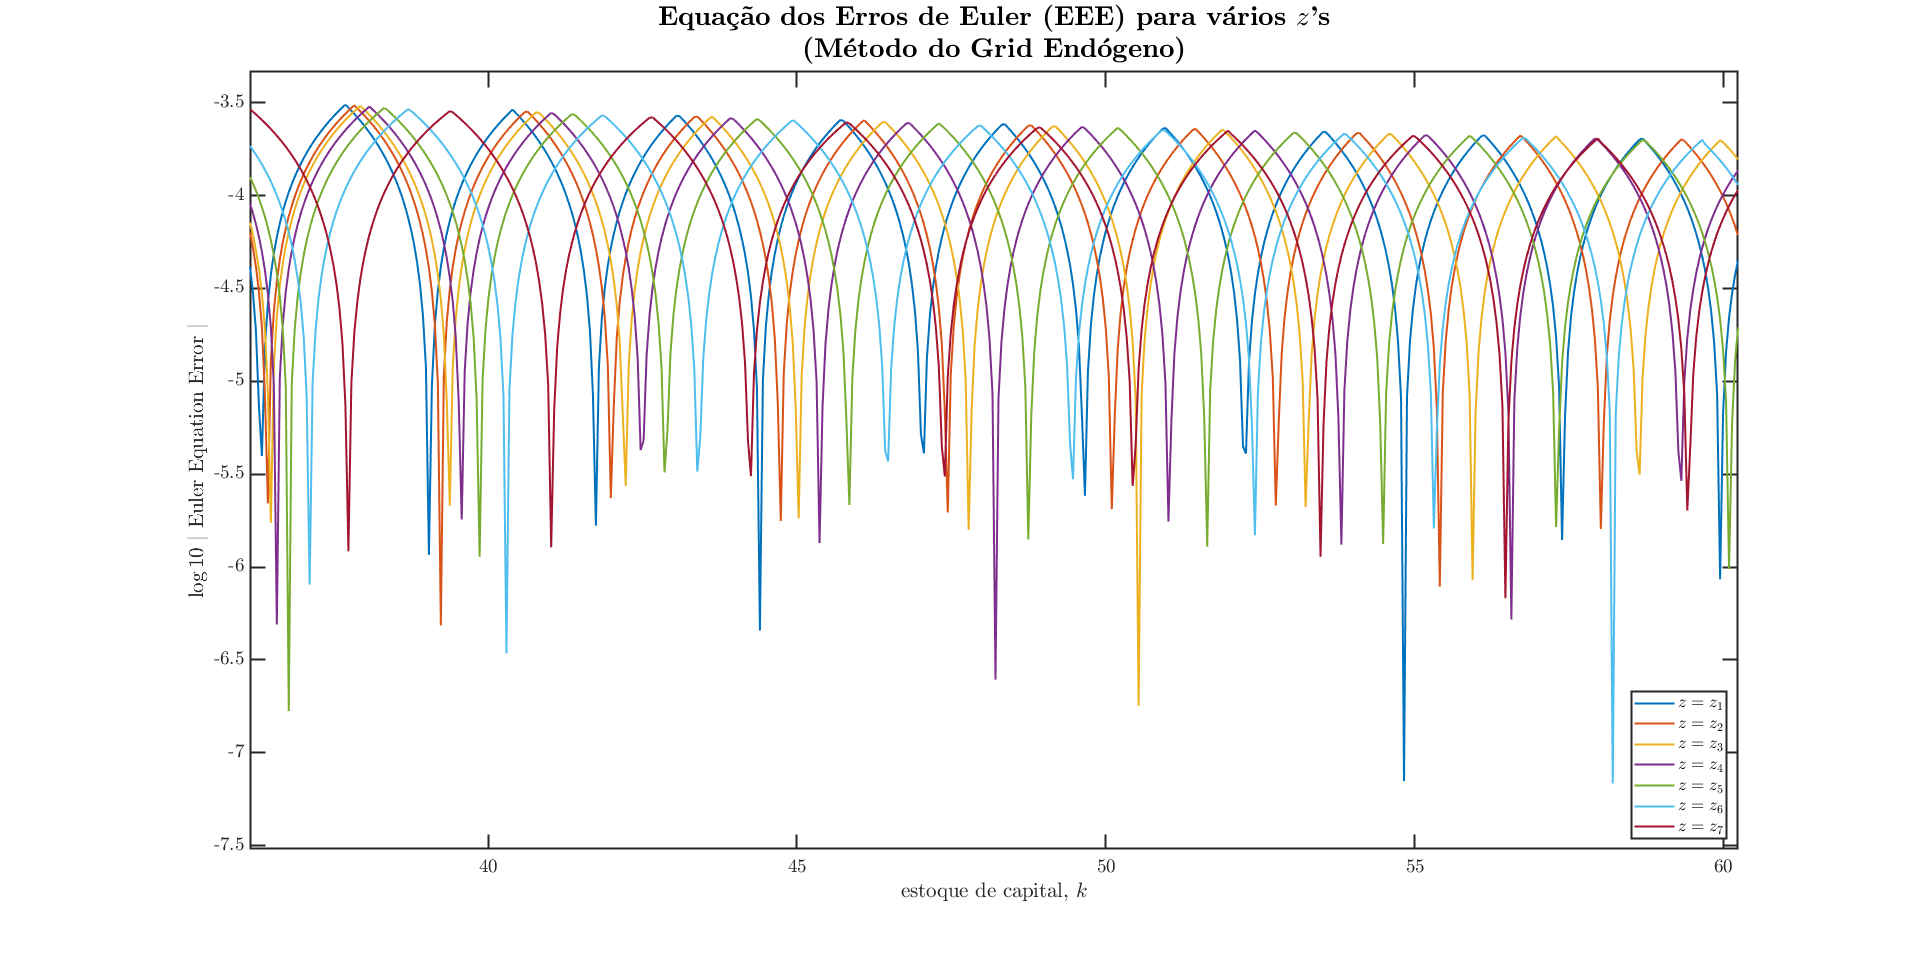
\includegraphics[scale=0.3]{eee_egm.png}
\caption{Erros de Euler (Grid Endógeno)}
\label{fig13}
\end{figure}\\
Sua amplitude vai de $-3.5101$ a $-7.1652$. O que, na nossa interpretação, significa que cometemos erros de $\$1$ a cada $\sim \$3236.68 - \$ 14,628,506.87$ gastos. Bem inferior aos modelos estimados anteriormente, mostrando ser uma estimação bem mais fiel.
\end{sol}

\end{enumerate}
\end{document}
